% Created by tikzDevice version 0.9 on 2016-01-12 22:38:35
% !TEX encoding = UTF-8 Unicode
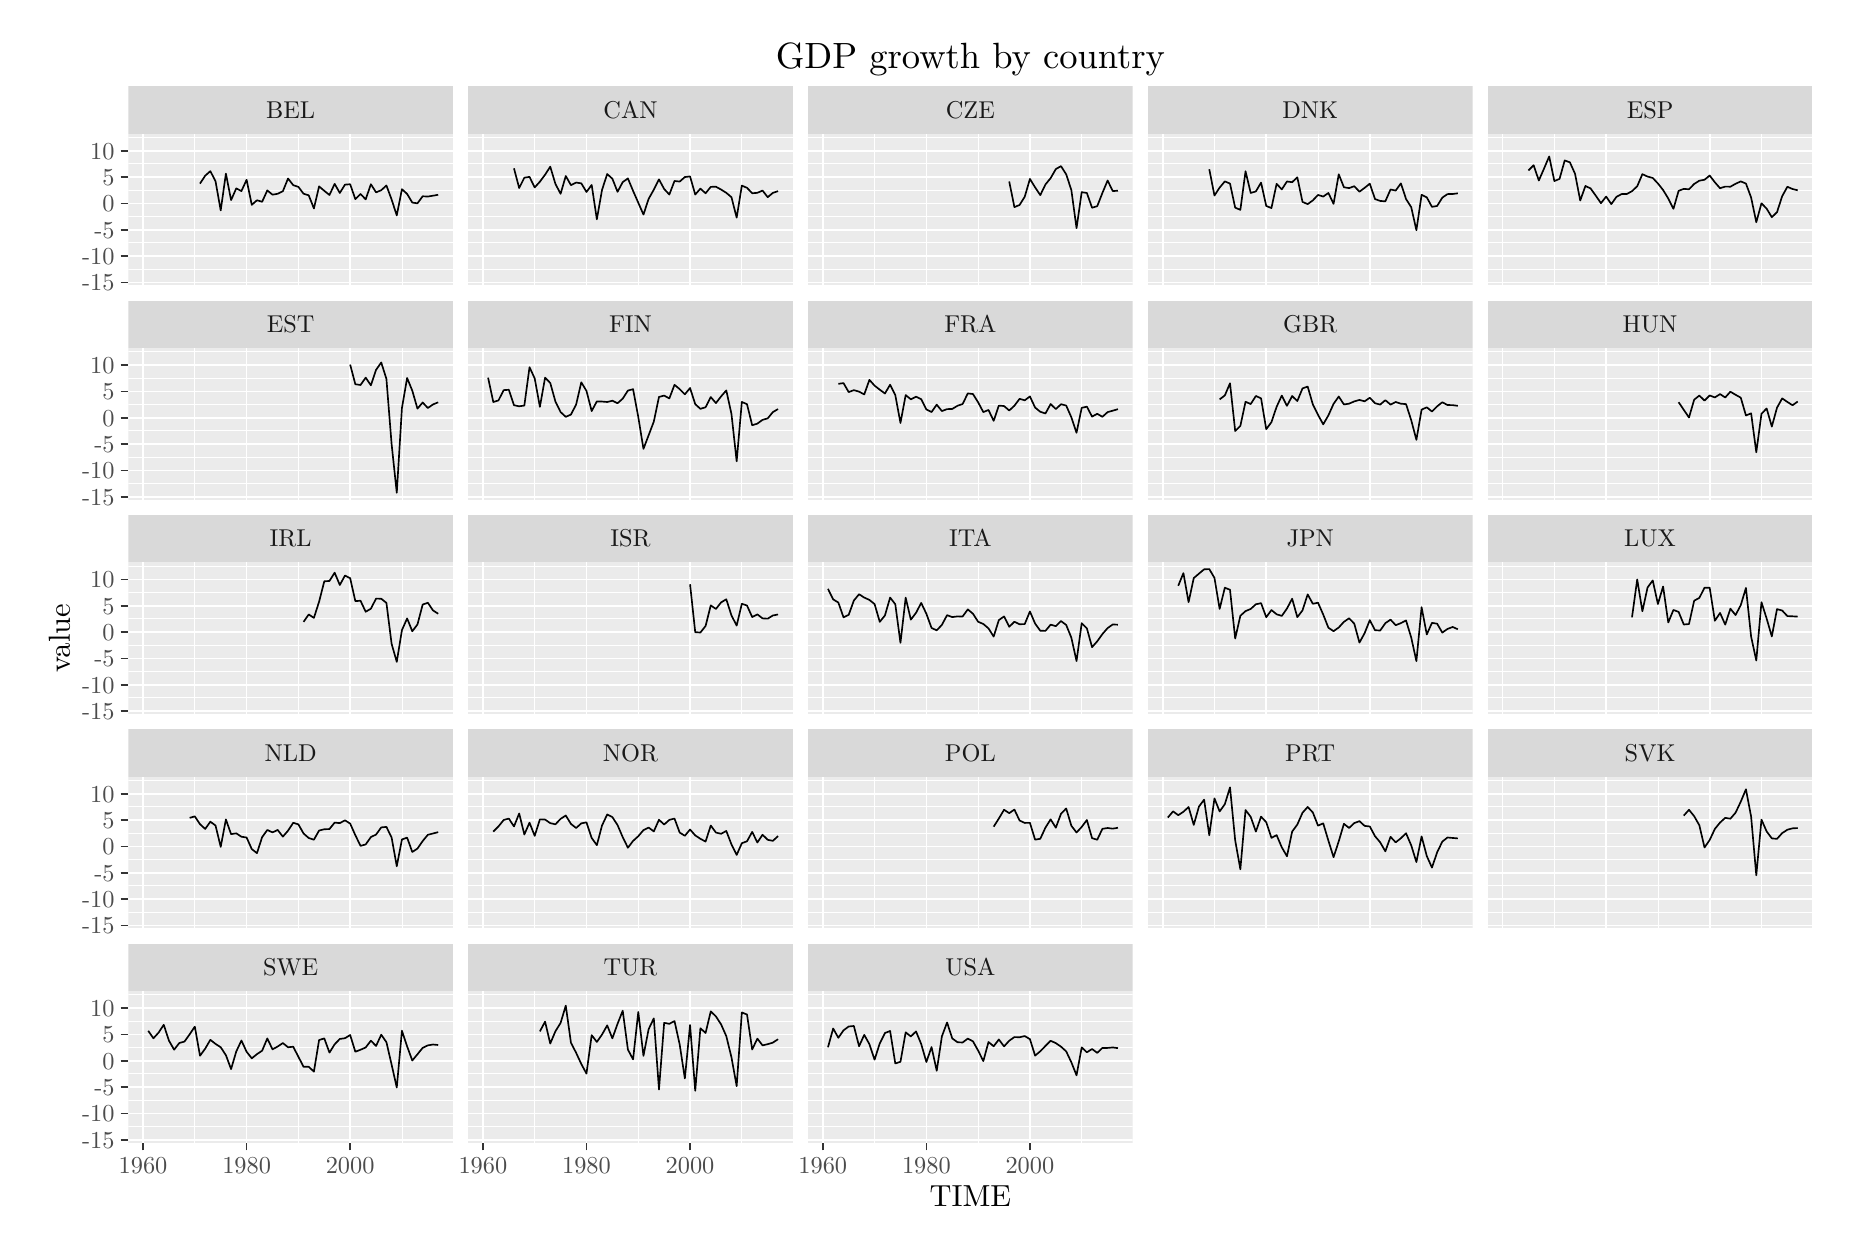
\begin{tikzpicture}[x=1pt,y=1pt]
\definecolor{fillColor}{RGB}{255,255,255}
\path[use as bounding box,fill=fillColor,fill opacity=0.00] (0,0) rectangle (650.43,433.62);
\begin{scope}
\path[clip] (  0.00,  0.00) rectangle (650.43,433.62);
\definecolor{drawColor}{RGB}{255,255,255}
\definecolor{fillColor}{RGB}{255,255,255}

\path[draw=drawColor,line width= 0.6pt,line join=round,line cap=round,fill=fillColor] (  0.00,  0.00) rectangle (650.43,433.62);
\end{scope}
\begin{scope}
\path[clip] ( 36.36,340.48) rectangle (153.67,395.37);
\definecolor{fillColor}{gray}{0.92}

\path[fill=fillColor] ( 36.36,340.48) rectangle (153.67,395.37);
\definecolor{drawColor}{RGB}{255,255,255}

\path[draw=drawColor,line width= 0.3pt,line join=round] ( 36.36,346.32) --
	(153.67,346.32);

\path[draw=drawColor,line width= 0.3pt,line join=round] ( 36.36,355.84) --
	(153.67,355.84);

\path[draw=drawColor,line width= 0.3pt,line join=round] ( 36.36,365.36) --
	(153.67,365.36);

\path[draw=drawColor,line width= 0.3pt,line join=round] ( 36.36,374.88) --
	(153.67,374.88);

\path[draw=drawColor,line width= 0.3pt,line join=round] ( 36.36,384.40) --
	(153.67,384.40);

\path[draw=drawColor,line width= 0.3pt,line join=round] ( 36.36,393.91) --
	(153.67,393.91);

\path[draw=drawColor,line width= 0.3pt,line join=round] ( 60.40,340.48) --
	( 60.40,395.37);

\path[draw=drawColor,line width= 0.3pt,line join=round] ( 97.82,340.48) --
	( 97.82,395.37);

\path[draw=drawColor,line width= 0.3pt,line join=round] (135.24,340.48) --
	(135.24,395.37);

\path[draw=drawColor,line width= 0.6pt,line join=round] ( 36.36,341.56) --
	(153.67,341.56);

\path[draw=drawColor,line width= 0.6pt,line join=round] ( 36.36,351.08) --
	(153.67,351.08);

\path[draw=drawColor,line width= 0.6pt,line join=round] ( 36.36,360.60) --
	(153.67,360.60);

\path[draw=drawColor,line width= 0.6pt,line join=round] ( 36.36,370.12) --
	(153.67,370.12);

\path[draw=drawColor,line width= 0.6pt,line join=round] ( 36.36,379.64) --
	(153.67,379.64);

\path[draw=drawColor,line width= 0.6pt,line join=round] ( 36.36,389.16) --
	(153.67,389.16);

\path[draw=drawColor,line width= 0.6pt,line join=round] ( 41.69,340.48) --
	( 41.69,395.37);

\path[draw=drawColor,line width= 0.6pt,line join=round] ( 79.11,340.48) --
	( 79.11,395.37);

\path[draw=drawColor,line width= 0.6pt,line join=round] (116.53,340.48) --
	(116.53,395.37);
\definecolor{drawColor}{RGB}{0,0,0}

\path[draw=drawColor,line width= 0.6pt,line join=round] ( 62.27,377.26) --
	( 64.14,380.12) --
	( 66.01,381.77) --
	( 67.88,378.11) --
	( 69.75,367.59) --
	( 71.63,380.88) --
	( 73.50,371.31) --
	( 75.37,375.53) --
	( 77.24,374.58) --
	( 79.11,378.65) --
	( 80.98,369.59) --
	( 82.85,371.25) --
	( 84.72,370.71) --
	( 86.59,374.81) --
	( 88.47,373.26) --
	( 90.34,373.59) --
	( 92.21,374.51) --
	( 94.08,379.11) --
	( 95.95,376.72) --
	( 97.82,376.09) --
	( 99.69,373.61) --
	(101.56,373.03) --
	(103.43,368.29) --
	(105.30,376.26) --
	(107.18,374.66) --
	(109.05,373.15) --
	(110.92,377.18) --
	(112.79,373.88) --
	(114.66,376.90) --
	(116.53,377.04) --
	(118.40,371.66) --
	(120.27,373.51) --
	(122.14,371.59) --
	(124.02,377.04) --
	(125.89,374.11) --
	(127.76,374.88) --
	(129.63,376.59) --
	(131.50,371.54) --
	(133.37,365.77) --
	(135.24,375.25) --
	(137.11,373.54) --
	(138.98,370.41) --
	(140.85,370.15) --
	(142.73,372.69) --
	(144.60,372.59) --
	(146.47,372.90) --
	(148.34,373.23);
\end{scope}
\begin{scope}
\path[clip] (159.17,340.48) rectangle (276.49,395.37);
\definecolor{fillColor}{gray}{0.92}

\path[fill=fillColor] (159.17,340.48) rectangle (276.49,395.37);
\definecolor{drawColor}{RGB}{255,255,255}

\path[draw=drawColor,line width= 0.3pt,line join=round] (159.17,346.32) --
	(276.49,346.32);

\path[draw=drawColor,line width= 0.3pt,line join=round] (159.17,355.84) --
	(276.49,355.84);

\path[draw=drawColor,line width= 0.3pt,line join=round] (159.17,365.36) --
	(276.49,365.36);

\path[draw=drawColor,line width= 0.3pt,line join=round] (159.17,374.88) --
	(276.49,374.88);

\path[draw=drawColor,line width= 0.3pt,line join=round] (159.17,384.40) --
	(276.49,384.40);

\path[draw=drawColor,line width= 0.3pt,line join=round] (159.17,393.91) --
	(276.49,393.91);

\path[draw=drawColor,line width= 0.3pt,line join=round] (183.21,340.48) --
	(183.21,395.37);

\path[draw=drawColor,line width= 0.3pt,line join=round] (220.64,340.48) --
	(220.64,395.37);

\path[draw=drawColor,line width= 0.3pt,line join=round] (258.06,340.48) --
	(258.06,395.37);

\path[draw=drawColor,line width= 0.6pt,line join=round] (159.17,341.56) --
	(276.49,341.56);

\path[draw=drawColor,line width= 0.6pt,line join=round] (159.17,351.08) --
	(276.49,351.08);

\path[draw=drawColor,line width= 0.6pt,line join=round] (159.17,360.60) --
	(276.49,360.60);

\path[draw=drawColor,line width= 0.6pt,line join=round] (159.17,370.12) --
	(276.49,370.12);

\path[draw=drawColor,line width= 0.6pt,line join=round] (159.17,379.64) --
	(276.49,379.64);

\path[draw=drawColor,line width= 0.6pt,line join=round] (159.17,389.16) --
	(276.49,389.16);

\path[draw=drawColor,line width= 0.6pt,line join=round] (164.50,340.48) --
	(164.50,395.37);

\path[draw=drawColor,line width= 0.6pt,line join=round] (201.92,340.48) --
	(201.92,395.37);

\path[draw=drawColor,line width= 0.6pt,line join=round] (239.35,340.48) --
	(239.35,395.37);
\definecolor{drawColor}{RGB}{0,0,0}

\path[draw=drawColor,line width= 0.6pt,line join=round] (175.73,382.77) --
	(177.60,375.67) --
	(179.47,379.41) --
	(181.34,379.70) --
	(183.21,375.89) --
	(185.09,377.96) --
	(186.96,380.49) --
	(188.83,383.38) --
	(190.70,377.15) --
	(192.57,373.59) --
	(194.44,380.02) --
	(196.31,376.70) --
	(198.18,377.65) --
	(200.05,377.36) --
	(201.92,374.24) --
	(203.80,376.79) --
	(205.67,364.37) --
	(207.54,375.00) --
	(209.41,380.73) --
	(211.28,379.03) --
	(213.15,374.30) --
	(215.02,377.81) --
	(216.89,379.14) --
	(218.76,374.64) --
	(220.64,370.36) --
	(222.51,366.08) --
	(224.38,371.75) --
	(226.25,375.08) --
	(228.12,378.79) --
	(229.99,375.33) --
	(231.86,373.32) --
	(233.73,378.22) --
	(235.60,378.00) --
	(237.47,379.63) --
	(239.35,379.87) --
	(241.22,373.33) --
	(243.09,375.45) --
	(244.96,373.78) --
	(246.83,376.09) --
	(248.70,376.14) --
	(250.57,375.11) --
	(252.44,373.94) --
	(254.31,372.36) --
	(256.19,364.96) --
	(258.06,376.54) --
	(259.93,375.75) --
	(261.80,373.78) --
	(263.67,373.93) --
	(265.54,374.76) --
	(267.41,372.36) --
	(269.28,373.92) --
	(271.15,374.55);
\end{scope}
\begin{scope}
\path[clip] (281.99,340.48) rectangle (399.30,395.37);
\definecolor{fillColor}{gray}{0.92}

\path[fill=fillColor] (281.99,340.48) rectangle (399.30,395.37);
\definecolor{drawColor}{RGB}{255,255,255}

\path[draw=drawColor,line width= 0.3pt,line join=round] (281.99,346.32) --
	(399.30,346.32);

\path[draw=drawColor,line width= 0.3pt,line join=round] (281.99,355.84) --
	(399.30,355.84);

\path[draw=drawColor,line width= 0.3pt,line join=round] (281.99,365.36) --
	(399.30,365.36);

\path[draw=drawColor,line width= 0.3pt,line join=round] (281.99,374.88) --
	(399.30,374.88);

\path[draw=drawColor,line width= 0.3pt,line join=round] (281.99,384.40) --
	(399.30,384.40);

\path[draw=drawColor,line width= 0.3pt,line join=round] (281.99,393.91) --
	(399.30,393.91);

\path[draw=drawColor,line width= 0.3pt,line join=round] (306.03,340.48) --
	(306.03,395.37);

\path[draw=drawColor,line width= 0.3pt,line join=round] (343.45,340.48) --
	(343.45,395.37);

\path[draw=drawColor,line width= 0.3pt,line join=round] (380.87,340.48) --
	(380.87,395.37);

\path[draw=drawColor,line width= 0.6pt,line join=round] (281.99,341.56) --
	(399.30,341.56);

\path[draw=drawColor,line width= 0.6pt,line join=round] (281.99,351.08) --
	(399.30,351.08);

\path[draw=drawColor,line width= 0.6pt,line join=round] (281.99,360.60) --
	(399.30,360.60);

\path[draw=drawColor,line width= 0.6pt,line join=round] (281.99,370.12) --
	(399.30,370.12);

\path[draw=drawColor,line width= 0.6pt,line join=round] (281.99,379.64) --
	(399.30,379.64);

\path[draw=drawColor,line width= 0.6pt,line join=round] (281.99,389.16) --
	(399.30,389.16);

\path[draw=drawColor,line width= 0.6pt,line join=round] (287.32,340.48) --
	(287.32,395.37);

\path[draw=drawColor,line width= 0.6pt,line join=round] (324.74,340.48) --
	(324.74,395.37);

\path[draw=drawColor,line width= 0.6pt,line join=round] (362.16,340.48) --
	(362.16,395.37);
\definecolor{drawColor}{RGB}{0,0,0}

\path[draw=drawColor,line width= 0.6pt,line join=round] (354.68,378.04) --
	(356.55,368.78) --
	(358.42,369.54) --
	(360.29,372.54) --
	(362.16,378.96) --
	(364.03,375.91) --
	(365.90,373.09) --
	(367.77,376.97) --
	(369.64,379.24) --
	(371.52,382.52) --
	(373.39,383.58) --
	(375.26,380.62) --
	(377.13,374.95) --
	(379.00,361.17) --
	(380.87,374.19) --
	(382.74,373.87) --
	(384.61,368.55) --
	(386.48,369.11) --
	(388.35,373.89) --
	(390.23,378.39) --
	(392.10,374.56) --
	(393.97,374.71);
\end{scope}
\begin{scope}
\path[clip] (404.80,340.48) rectangle (522.12,395.37);
\definecolor{fillColor}{gray}{0.92}

\path[fill=fillColor] (404.80,340.48) rectangle (522.12,395.37);
\definecolor{drawColor}{RGB}{255,255,255}

\path[draw=drawColor,line width= 0.3pt,line join=round] (404.80,346.32) --
	(522.12,346.32);

\path[draw=drawColor,line width= 0.3pt,line join=round] (404.80,355.84) --
	(522.12,355.84);

\path[draw=drawColor,line width= 0.3pt,line join=round] (404.80,365.36) --
	(522.12,365.36);

\path[draw=drawColor,line width= 0.3pt,line join=round] (404.80,374.88) --
	(522.12,374.88);

\path[draw=drawColor,line width= 0.3pt,line join=round] (404.80,384.40) --
	(522.12,384.40);

\path[draw=drawColor,line width= 0.3pt,line join=round] (404.80,393.91) --
	(522.12,393.91);

\path[draw=drawColor,line width= 0.3pt,line join=round] (428.84,340.48) --
	(428.84,395.37);

\path[draw=drawColor,line width= 0.3pt,line join=round] (466.26,340.48) --
	(466.26,395.37);

\path[draw=drawColor,line width= 0.3pt,line join=round] (503.69,340.48) --
	(503.69,395.37);

\path[draw=drawColor,line width= 0.6pt,line join=round] (404.80,341.56) --
	(522.12,341.56);

\path[draw=drawColor,line width= 0.6pt,line join=round] (404.80,351.08) --
	(522.12,351.08);

\path[draw=drawColor,line width= 0.6pt,line join=round] (404.80,360.60) --
	(522.12,360.60);

\path[draw=drawColor,line width= 0.6pt,line join=round] (404.80,370.12) --
	(522.12,370.12);

\path[draw=drawColor,line width= 0.6pt,line join=round] (404.80,379.64) --
	(522.12,379.64);

\path[draw=drawColor,line width= 0.6pt,line join=round] (404.80,389.16) --
	(522.12,389.16);

\path[draw=drawColor,line width= 0.6pt,line join=round] (410.13,340.48) --
	(410.13,395.37);

\path[draw=drawColor,line width= 0.6pt,line join=round] (447.55,340.48) --
	(447.55,395.37);

\path[draw=drawColor,line width= 0.6pt,line join=round] (484.97,340.48) --
	(484.97,395.37);
\definecolor{drawColor}{RGB}{0,0,0}

\path[draw=drawColor,line width= 0.6pt,line join=round] (426.97,382.45) --
	(428.84,372.97) --
	(430.71,375.83) --
	(432.59,378.07) --
	(434.46,377.28) --
	(436.33,368.57) --
	(438.20,367.79) --
	(440.07,381.72) --
	(441.94,373.89) --
	(443.81,374.45) --
	(445.68,377.64) --
	(447.55,369.19) --
	(449.43,368.43) --
	(451.30,377.19) --
	(453.17,375.17) --
	(455.04,378.05) --
	(456.91,377.78) --
	(458.78,379.54) --
	(460.65,370.67) --
	(462.52,369.85) --
	(464.39,371.21) --
	(466.26,373.18) --
	(468.14,372.59) --
	(470.01,373.88) --
	(471.88,369.95) --
	(473.75,380.64) --
	(475.62,375.95) --
	(477.49,375.64) --
	(479.36,376.33) --
	(481.23,374.34) --
	(483.10,375.73) --
	(484.97,377.25) --
	(486.85,371.69) --
	(488.72,371.01) --
	(490.59,370.86) --
	(492.46,375.14) --
	(494.33,374.76) --
	(496.20,377.35) --
	(498.07,371.69) --
	(499.94,368.75) --
	(501.81,360.43) --
	(503.69,373.21) --
	(505.56,372.31) --
	(507.43,368.87) --
	(509.30,369.19) --
	(511.17,372.19) --
	(513.04,373.48) --
	(514.91,373.51) --
	(516.78,373.76);
\end{scope}
\begin{scope}
\path[clip] (527.62,340.48) rectangle (644.93,395.37);
\definecolor{fillColor}{gray}{0.92}

\path[fill=fillColor] (527.62,340.48) rectangle (644.93,395.37);
\definecolor{drawColor}{RGB}{255,255,255}

\path[draw=drawColor,line width= 0.3pt,line join=round] (527.62,346.32) --
	(644.93,346.32);

\path[draw=drawColor,line width= 0.3pt,line join=round] (527.62,355.84) --
	(644.93,355.84);

\path[draw=drawColor,line width= 0.3pt,line join=round] (527.62,365.36) --
	(644.93,365.36);

\path[draw=drawColor,line width= 0.3pt,line join=round] (527.62,374.88) --
	(644.93,374.88);

\path[draw=drawColor,line width= 0.3pt,line join=round] (527.62,384.40) --
	(644.93,384.40);

\path[draw=drawColor,line width= 0.3pt,line join=round] (527.62,393.91) --
	(644.93,393.91);

\path[draw=drawColor,line width= 0.3pt,line join=round] (551.66,340.48) --
	(551.66,395.37);

\path[draw=drawColor,line width= 0.3pt,line join=round] (589.08,340.48) --
	(589.08,395.37);

\path[draw=drawColor,line width= 0.3pt,line join=round] (626.50,340.48) --
	(626.50,395.37);

\path[draw=drawColor,line width= 0.6pt,line join=round] (527.62,341.56) --
	(644.93,341.56);

\path[draw=drawColor,line width= 0.6pt,line join=round] (527.62,351.08) --
	(644.93,351.08);

\path[draw=drawColor,line width= 0.6pt,line join=round] (527.62,360.60) --
	(644.93,360.60);

\path[draw=drawColor,line width= 0.6pt,line join=round] (527.62,370.12) --
	(644.93,370.12);

\path[draw=drawColor,line width= 0.6pt,line join=round] (527.62,379.64) --
	(644.93,379.64);

\path[draw=drawColor,line width= 0.6pt,line join=round] (527.62,389.16) --
	(644.93,389.16);

\path[draw=drawColor,line width= 0.6pt,line join=round] (532.95,340.48) --
	(532.95,395.37);

\path[draw=drawColor,line width= 0.6pt,line join=round] (570.37,340.48) --
	(570.37,395.37);

\path[draw=drawColor,line width= 0.6pt,line join=round] (607.79,340.48) --
	(607.79,395.37);
\definecolor{drawColor}{RGB}{0,0,0}

\path[draw=drawColor,line width= 0.6pt,line join=round] (542.30,382.02) --
	(544.17,383.91) --
	(546.05,378.38) --
	(547.92,382.68) --
	(549.79,387.08) --
	(551.66,378.20) --
	(553.53,378.96) --
	(555.40,385.63) --
	(557.27,384.96) --
	(559.14,380.81) --
	(561.01,371.15) --
	(562.88,376.41) --
	(564.76,375.52) --
	(566.63,372.90) --
	(568.50,370.20) --
	(570.37,372.59) --
	(572.24,369.86) --
	(574.11,372.49) --
	(575.98,373.49) --
	(577.85,373.51) --
	(579.72,374.54) --
	(581.60,376.31) --
	(583.47,380.68) --
	(585.34,379.81) --
	(587.21,379.31) --
	(589.08,377.32) --
	(590.95,374.96) --
	(592.82,371.89) --
	(594.69,368.16) --
	(596.56,374.65) --
	(598.43,375.37) --
	(600.31,375.21) --
	(602.18,377.14) --
	(604.05,378.32) --
	(605.92,378.66) --
	(607.79,380.19) --
	(609.66,377.74) --
	(611.53,375.60) --
	(613.40,376.19) --
	(615.27,376.15) --
	(617.14,377.21) --
	(619.02,378.06) --
	(620.89,377.29) --
	(622.76,372.24) --
	(624.63,363.32) --
	(626.50,370.15) --
	(628.37,368.22) --
	(630.24,365.13) --
	(632.11,366.94) --
	(633.98,372.71) --
	(635.86,376.13) --
	(637.73,375.31) --
	(639.60,374.85);
\end{scope}
\begin{scope}
\path[clip] ( 36.36,263.03) rectangle (153.67,317.92);
\definecolor{fillColor}{gray}{0.92}

\path[fill=fillColor] ( 36.36,263.03) rectangle (153.67,317.92);
\definecolor{drawColor}{RGB}{255,255,255}

\path[draw=drawColor,line width= 0.3pt,line join=round] ( 36.36,268.88) --
	(153.67,268.88);

\path[draw=drawColor,line width= 0.3pt,line join=round] ( 36.36,278.39) --
	(153.67,278.39);

\path[draw=drawColor,line width= 0.3pt,line join=round] ( 36.36,287.91) --
	(153.67,287.91);

\path[draw=drawColor,line width= 0.3pt,line join=round] ( 36.36,297.43) --
	(153.67,297.43);

\path[draw=drawColor,line width= 0.3pt,line join=round] ( 36.36,306.95) --
	(153.67,306.95);

\path[draw=drawColor,line width= 0.3pt,line join=round] ( 36.36,316.47) --
	(153.67,316.47);

\path[draw=drawColor,line width= 0.3pt,line join=round] ( 60.40,263.03) --
	( 60.40,317.92);

\path[draw=drawColor,line width= 0.3pt,line join=round] ( 97.82,263.03) --
	( 97.82,317.92);

\path[draw=drawColor,line width= 0.3pt,line join=round] (135.24,263.03) --
	(135.24,317.92);

\path[draw=drawColor,line width= 0.6pt,line join=round] ( 36.36,264.12) --
	(153.67,264.12);

\path[draw=drawColor,line width= 0.6pt,line join=round] ( 36.36,273.63) --
	(153.67,273.63);

\path[draw=drawColor,line width= 0.6pt,line join=round] ( 36.36,283.15) --
	(153.67,283.15);

\path[draw=drawColor,line width= 0.6pt,line join=round] ( 36.36,292.67) --
	(153.67,292.67);

\path[draw=drawColor,line width= 0.6pt,line join=round] ( 36.36,302.19) --
	(153.67,302.19);

\path[draw=drawColor,line width= 0.6pt,line join=round] ( 36.36,311.71) --
	(153.67,311.71);

\path[draw=drawColor,line width= 0.6pt,line join=round] ( 41.69,263.03) --
	( 41.69,317.92);

\path[draw=drawColor,line width= 0.6pt,line join=round] ( 79.11,263.03) --
	( 79.11,317.92);

\path[draw=drawColor,line width= 0.6pt,line join=round] (116.53,263.03) --
	(116.53,317.92);
\definecolor{drawColor}{RGB}{0,0,0}

\path[draw=drawColor,line width= 0.6pt,line join=round] (116.53,311.87) --
	(118.40,304.77) --
	(120.27,304.50) --
	(122.14,307.15) --
	(124.02,304.39) --
	(125.89,309.97) --
	(127.76,312.63) --
	(129.63,306.70) --
	(131.50,283.20) --
	(133.37,265.53) --
	(135.24,296.17) --
	(137.11,307.03) --
	(138.98,302.44) --
	(140.85,295.95) --
	(142.73,298.18) --
	(144.60,296.17) --
	(146.47,297.48) --
	(148.34,298.24);
\end{scope}
\begin{scope}
\path[clip] (159.17,263.03) rectangle (276.49,317.92);
\definecolor{fillColor}{gray}{0.92}

\path[fill=fillColor] (159.17,263.03) rectangle (276.49,317.92);
\definecolor{drawColor}{RGB}{255,255,255}

\path[draw=drawColor,line width= 0.3pt,line join=round] (159.17,268.88) --
	(276.49,268.88);

\path[draw=drawColor,line width= 0.3pt,line join=round] (159.17,278.39) --
	(276.49,278.39);

\path[draw=drawColor,line width= 0.3pt,line join=round] (159.17,287.91) --
	(276.49,287.91);

\path[draw=drawColor,line width= 0.3pt,line join=round] (159.17,297.43) --
	(276.49,297.43);

\path[draw=drawColor,line width= 0.3pt,line join=round] (159.17,306.95) --
	(276.49,306.95);

\path[draw=drawColor,line width= 0.3pt,line join=round] (159.17,316.47) --
	(276.49,316.47);

\path[draw=drawColor,line width= 0.3pt,line join=round] (183.21,263.03) --
	(183.21,317.92);

\path[draw=drawColor,line width= 0.3pt,line join=round] (220.64,263.03) --
	(220.64,317.92);

\path[draw=drawColor,line width= 0.3pt,line join=round] (258.06,263.03) --
	(258.06,317.92);

\path[draw=drawColor,line width= 0.6pt,line join=round] (159.17,264.12) --
	(276.49,264.12);

\path[draw=drawColor,line width= 0.6pt,line join=round] (159.17,273.63) --
	(276.49,273.63);

\path[draw=drawColor,line width= 0.6pt,line join=round] (159.17,283.15) --
	(276.49,283.15);

\path[draw=drawColor,line width= 0.6pt,line join=round] (159.17,292.67) --
	(276.49,292.67);

\path[draw=drawColor,line width= 0.6pt,line join=round] (159.17,302.19) --
	(276.49,302.19);

\path[draw=drawColor,line width= 0.6pt,line join=round] (159.17,311.71) --
	(276.49,311.71);

\path[draw=drawColor,line width= 0.6pt,line join=round] (164.50,263.03) --
	(164.50,317.92);

\path[draw=drawColor,line width= 0.6pt,line join=round] (201.92,263.03) --
	(201.92,317.92);

\path[draw=drawColor,line width= 0.6pt,line join=round] (239.35,263.03) --
	(239.35,317.92);
\definecolor{drawColor}{RGB}{0,0,0}

\path[draw=drawColor,line width= 0.6pt,line join=round] (166.37,307.15) --
	(168.25,298.35) --
	(170.12,298.92) --
	(171.99,302.64) --
	(173.86,302.77) --
	(175.73,297.19) --
	(177.60,296.80) --
	(179.47,297.06) --
	(181.34,310.93) --
	(183.21,306.89) --
	(185.09,296.60) --
	(186.96,307.14) --
	(188.83,305.24) --
	(190.70,298.52) --
	(192.57,294.71) --
	(194.44,292.99) --
	(196.31,293.82) --
	(198.18,297.43) --
	(200.05,305.47) --
	(201.92,302.36) --
	(203.80,295.09) --
	(205.67,298.57) --
	(207.54,298.51) --
	(209.41,298.36) --
	(211.28,298.81) --
	(213.15,297.91) --
	(215.02,299.56) --
	(216.89,302.48) --
	(218.76,302.98) --
	(220.64,292.94) --
	(222.51,281.41) --
	(224.38,286.34) --
	(226.25,291.27) --
	(228.12,300.17) --
	(229.99,300.68) --
	(231.86,299.63) --
	(233.73,304.57) --
	(235.60,303.00) --
	(237.47,301.13) --
	(239.35,303.40) --
	(241.22,297.58) --
	(243.09,295.87) --
	(244.96,296.47) --
	(246.83,300.14) --
	(248.70,297.96) --
	(250.57,300.39) --
	(252.44,302.54) --
	(254.31,294.04) --
	(256.19,276.93) --
	(258.06,298.37) --
	(259.93,297.56) --
	(261.80,289.96) --
	(263.67,290.54) --
	(265.54,291.90) --
	(267.41,292.44) --
	(269.28,294.70) --
	(271.15,295.81);
\end{scope}
\begin{scope}
\path[clip] (281.99,263.03) rectangle (399.30,317.92);
\definecolor{fillColor}{gray}{0.92}

\path[fill=fillColor] (281.99,263.03) rectangle (399.30,317.92);
\definecolor{drawColor}{RGB}{255,255,255}

\path[draw=drawColor,line width= 0.3pt,line join=round] (281.99,268.88) --
	(399.30,268.88);

\path[draw=drawColor,line width= 0.3pt,line join=round] (281.99,278.39) --
	(399.30,278.39);

\path[draw=drawColor,line width= 0.3pt,line join=round] (281.99,287.91) --
	(399.30,287.91);

\path[draw=drawColor,line width= 0.3pt,line join=round] (281.99,297.43) --
	(399.30,297.43);

\path[draw=drawColor,line width= 0.3pt,line join=round] (281.99,306.95) --
	(399.30,306.95);

\path[draw=drawColor,line width= 0.3pt,line join=round] (281.99,316.47) --
	(399.30,316.47);

\path[draw=drawColor,line width= 0.3pt,line join=round] (306.03,263.03) --
	(306.03,317.92);

\path[draw=drawColor,line width= 0.3pt,line join=round] (343.45,263.03) --
	(343.45,317.92);

\path[draw=drawColor,line width= 0.3pt,line join=round] (380.87,263.03) --
	(380.87,317.92);

\path[draw=drawColor,line width= 0.6pt,line join=round] (281.99,264.12) --
	(399.30,264.12);

\path[draw=drawColor,line width= 0.6pt,line join=round] (281.99,273.63) --
	(399.30,273.63);

\path[draw=drawColor,line width= 0.6pt,line join=round] (281.99,283.15) --
	(399.30,283.15);

\path[draw=drawColor,line width= 0.6pt,line join=round] (281.99,292.67) --
	(399.30,292.67);

\path[draw=drawColor,line width= 0.6pt,line join=round] (281.99,302.19) --
	(399.30,302.19);

\path[draw=drawColor,line width= 0.6pt,line join=round] (281.99,311.71) --
	(399.30,311.71);

\path[draw=drawColor,line width= 0.6pt,line join=round] (287.32,263.03) --
	(287.32,317.92);

\path[draw=drawColor,line width= 0.6pt,line join=round] (324.74,263.03) --
	(324.74,317.92);

\path[draw=drawColor,line width= 0.6pt,line join=round] (362.16,263.03) --
	(362.16,317.92);
\definecolor{drawColor}{RGB}{0,0,0}

\path[draw=drawColor,line width= 0.6pt,line join=round] (292.93,304.91) --
	(294.80,305.18) --
	(296.67,301.93) --
	(298.54,302.64) --
	(300.42,302.10) --
	(302.29,301.08) --
	(304.16,306.35) --
	(306.03,304.26) --
	(307.90,302.80) --
	(309.77,301.43) --
	(311.64,304.60) --
	(313.51,300.86) --
	(315.38,290.78) --
	(317.26,300.85) --
	(319.13,299.32) --
	(321.00,300.27) --
	(322.87,299.37) --
	(324.74,295.67) --
	(326.61,294.72) --
	(328.48,297.39) --
	(330.35,295.07) --
	(332.22,295.78) --
	(334.09,295.84) --
	(335.97,296.98) --
	(337.84,297.62) --
	(339.71,301.46) --
	(341.58,301.22) --
	(343.45,298.23) --
	(345.32,294.71) --
	(347.19,295.47) --
	(349.06,291.55) --
	(350.93,297.06) --
	(352.81,296.89) --
	(354.68,295.28) --
	(356.55,297.01) --
	(358.42,299.50) --
	(360.29,298.97) --
	(362.16,300.36) --
	(364.03,296.34) --
	(365.90,294.82) --
	(367.77,294.21) --
	(369.64,297.61) --
	(371.52,295.79) --
	(373.39,297.55) --
	(375.26,297.07) --
	(377.13,292.84) --
	(379.00,287.24) --
	(380.87,296.25) --
	(382.74,296.66) --
	(384.61,293.08) --
	(386.48,294.09) --
	(388.35,293.00) --
	(390.23,294.70) --
	(392.10,295.22) --
	(393.97,295.76);
\end{scope}
\begin{scope}
\path[clip] (404.80,263.03) rectangle (522.12,317.92);
\definecolor{fillColor}{gray}{0.92}

\path[fill=fillColor] (404.80,263.03) rectangle (522.12,317.92);
\definecolor{drawColor}{RGB}{255,255,255}

\path[draw=drawColor,line width= 0.3pt,line join=round] (404.80,268.88) --
	(522.12,268.88);

\path[draw=drawColor,line width= 0.3pt,line join=round] (404.80,278.39) --
	(522.12,278.39);

\path[draw=drawColor,line width= 0.3pt,line join=round] (404.80,287.91) --
	(522.12,287.91);

\path[draw=drawColor,line width= 0.3pt,line join=round] (404.80,297.43) --
	(522.12,297.43);

\path[draw=drawColor,line width= 0.3pt,line join=round] (404.80,306.95) --
	(522.12,306.95);

\path[draw=drawColor,line width= 0.3pt,line join=round] (404.80,316.47) --
	(522.12,316.47);

\path[draw=drawColor,line width= 0.3pt,line join=round] (428.84,263.03) --
	(428.84,317.92);

\path[draw=drawColor,line width= 0.3pt,line join=round] (466.26,263.03) --
	(466.26,317.92);

\path[draw=drawColor,line width= 0.3pt,line join=round] (503.69,263.03) --
	(503.69,317.92);

\path[draw=drawColor,line width= 0.6pt,line join=round] (404.80,264.12) --
	(522.12,264.12);

\path[draw=drawColor,line width= 0.6pt,line join=round] (404.80,273.63) --
	(522.12,273.63);

\path[draw=drawColor,line width= 0.6pt,line join=round] (404.80,283.15) --
	(522.12,283.15);

\path[draw=drawColor,line width= 0.6pt,line join=round] (404.80,292.67) --
	(522.12,292.67);

\path[draw=drawColor,line width= 0.6pt,line join=round] (404.80,302.19) --
	(522.12,302.19);

\path[draw=drawColor,line width= 0.6pt,line join=round] (404.80,311.71) --
	(522.12,311.71);

\path[draw=drawColor,line width= 0.6pt,line join=round] (410.13,263.03) --
	(410.13,317.92);

\path[draw=drawColor,line width= 0.6pt,line join=round] (447.55,263.03) --
	(447.55,317.92);

\path[draw=drawColor,line width= 0.6pt,line join=round] (484.97,263.03) --
	(484.97,317.92);
\definecolor{drawColor}{RGB}{0,0,0}

\path[draw=drawColor,line width= 0.6pt,line join=round] (430.71,299.30) --
	(432.59,300.72) --
	(434.46,305.12) --
	(436.33,287.87) --
	(438.20,289.72) --
	(440.07,298.44) --
	(441.94,297.61) --
	(443.81,300.53) --
	(445.68,299.67) --
	(447.55,288.54) --
	(449.43,291.06) --
	(451.30,296.62) --
	(453.17,300.67) --
	(455.04,296.97) --
	(456.91,300.50) --
	(458.78,298.70) --
	(460.65,303.25) --
	(462.52,303.94) --
	(464.39,297.47) --
	(466.26,293.72) --
	(468.14,290.28) --
	(470.01,293.52) --
	(471.88,297.69) --
	(473.75,300.33) --
	(475.62,297.47) --
	(477.49,297.75) --
	(479.36,298.57) --
	(481.23,299.10) --
	(483.10,298.60) --
	(484.97,299.90) --
	(486.85,297.92) --
	(488.72,297.42) --
	(490.59,299.02) --
	(492.46,297.41) --
	(494.33,298.37) --
	(496.20,297.74) --
	(498.07,297.59) --
	(499.94,291.78) --
	(501.81,284.69) --
	(503.69,295.60) --
	(505.56,296.43) --
	(507.43,294.92) --
	(509.30,296.78) --
	(511.17,298.27) --
	(513.04,297.26) --
	(514.91,297.22) --
	(516.78,296.97);
\end{scope}
\begin{scope}
\path[clip] (527.62,263.03) rectangle (644.93,317.92);
\definecolor{fillColor}{gray}{0.92}

\path[fill=fillColor] (527.62,263.03) rectangle (644.93,317.92);
\definecolor{drawColor}{RGB}{255,255,255}

\path[draw=drawColor,line width= 0.3pt,line join=round] (527.62,268.88) --
	(644.93,268.88);

\path[draw=drawColor,line width= 0.3pt,line join=round] (527.62,278.39) --
	(644.93,278.39);

\path[draw=drawColor,line width= 0.3pt,line join=round] (527.62,287.91) --
	(644.93,287.91);

\path[draw=drawColor,line width= 0.3pt,line join=round] (527.62,297.43) --
	(644.93,297.43);

\path[draw=drawColor,line width= 0.3pt,line join=round] (527.62,306.95) --
	(644.93,306.95);

\path[draw=drawColor,line width= 0.3pt,line join=round] (527.62,316.47) --
	(644.93,316.47);

\path[draw=drawColor,line width= 0.3pt,line join=round] (551.66,263.03) --
	(551.66,317.92);

\path[draw=drawColor,line width= 0.3pt,line join=round] (589.08,263.03) --
	(589.08,317.92);

\path[draw=drawColor,line width= 0.3pt,line join=round] (626.50,263.03) --
	(626.50,317.92);

\path[draw=drawColor,line width= 0.6pt,line join=round] (527.62,264.12) --
	(644.93,264.12);

\path[draw=drawColor,line width= 0.6pt,line join=round] (527.62,273.63) --
	(644.93,273.63);

\path[draw=drawColor,line width= 0.6pt,line join=round] (527.62,283.15) --
	(644.93,283.15);

\path[draw=drawColor,line width= 0.6pt,line join=round] (527.62,292.67) --
	(644.93,292.67);

\path[draw=drawColor,line width= 0.6pt,line join=round] (527.62,302.19) --
	(644.93,302.19);

\path[draw=drawColor,line width= 0.6pt,line join=round] (527.62,311.71) --
	(644.93,311.71);

\path[draw=drawColor,line width= 0.6pt,line join=round] (532.95,263.03) --
	(532.95,317.92);

\path[draw=drawColor,line width= 0.6pt,line join=round] (570.37,263.03) --
	(570.37,317.92);

\path[draw=drawColor,line width= 0.6pt,line join=round] (607.79,263.03) --
	(607.79,317.92);
\definecolor{drawColor}{RGB}{0,0,0}

\path[draw=drawColor,line width= 0.6pt,line join=round] (596.56,298.28) --
	(598.43,295.51) --
	(600.31,292.75) --
	(602.18,299.19) --
	(604.05,300.68) --
	(605.92,298.85) --
	(607.79,300.72) --
	(609.66,300.00) --
	(611.53,301.20) --
	(613.40,299.99) --
	(615.27,302.07) --
	(617.14,300.96) --
	(619.02,299.92) --
	(620.89,293.48) --
	(622.76,294.27) --
	(624.63,280.18) --
	(626.50,294.09) --
	(628.37,296.02) --
	(630.24,289.46) --
	(632.11,296.27) --
	(633.98,299.66) --
	(635.86,298.37) --
	(637.73,297.17) --
	(639.60,298.53);
\end{scope}
\begin{scope}
\path[clip] ( 36.36,185.58) rectangle (153.67,240.47);
\definecolor{fillColor}{gray}{0.92}

\path[fill=fillColor] ( 36.36,185.58) rectangle (153.67,240.47);
\definecolor{drawColor}{RGB}{255,255,255}

\path[draw=drawColor,line width= 0.3pt,line join=round] ( 36.36,191.43) --
	(153.67,191.43);

\path[draw=drawColor,line width= 0.3pt,line join=round] ( 36.36,200.95) --
	(153.67,200.95);

\path[draw=drawColor,line width= 0.3pt,line join=round] ( 36.36,210.46) --
	(153.67,210.46);

\path[draw=drawColor,line width= 0.3pt,line join=round] ( 36.36,219.98) --
	(153.67,219.98);

\path[draw=drawColor,line width= 0.3pt,line join=round] ( 36.36,229.50) --
	(153.67,229.50);

\path[draw=drawColor,line width= 0.3pt,line join=round] ( 36.36,239.02) --
	(153.67,239.02);

\path[draw=drawColor,line width= 0.3pt,line join=round] ( 60.40,185.58) --
	( 60.40,240.47);

\path[draw=drawColor,line width= 0.3pt,line join=round] ( 97.82,185.58) --
	( 97.82,240.47);

\path[draw=drawColor,line width= 0.3pt,line join=round] (135.24,185.58) --
	(135.24,240.47);

\path[draw=drawColor,line width= 0.6pt,line join=round] ( 36.36,186.67) --
	(153.67,186.67);

\path[draw=drawColor,line width= 0.6pt,line join=round] ( 36.36,196.19) --
	(153.67,196.19);

\path[draw=drawColor,line width= 0.6pt,line join=round] ( 36.36,205.70) --
	(153.67,205.70);

\path[draw=drawColor,line width= 0.6pt,line join=round] ( 36.36,215.22) --
	(153.67,215.22);

\path[draw=drawColor,line width= 0.6pt,line join=round] ( 36.36,224.74) --
	(153.67,224.74);

\path[draw=drawColor,line width= 0.6pt,line join=round] ( 36.36,234.26) --
	(153.67,234.26);

\path[draw=drawColor,line width= 0.6pt,line join=round] ( 41.69,185.58) --
	( 41.69,240.47);

\path[draw=drawColor,line width= 0.6pt,line join=round] ( 79.11,185.58) --
	( 79.11,240.47);

\path[draw=drawColor,line width= 0.6pt,line join=round] (116.53,185.58) --
	(116.53,240.47);
\definecolor{drawColor}{RGB}{0,0,0}

\path[draw=drawColor,line width= 0.6pt,line join=round] ( 99.69,218.90) --
	(101.56,221.59) --
	(103.43,220.35) --
	(105.30,226.18) --
	(107.18,233.56) --
	(109.05,233.69) --
	(110.92,236.68) --
	(112.79,232.23) --
	(114.66,235.65) --
	(116.53,234.68) --
	(118.40,226.40) --
	(120.27,226.54) --
	(122.14,222.56) --
	(124.02,223.66) --
	(125.89,227.32) --
	(127.76,227.26) --
	(129.63,225.76) --
	(131.50,211.01) --
	(133.37,204.45) --
	(135.24,215.94) --
	(137.11,220.15) --
	(138.98,215.50) --
	(140.85,217.97) --
	(142.73,225.15) --
	(144.60,225.81) --
	(146.47,223.04) --
	(148.34,221.84);
\end{scope}
\begin{scope}
\path[clip] (159.17,185.58) rectangle (276.49,240.47);
\definecolor{fillColor}{gray}{0.92}

\path[fill=fillColor] (159.17,185.58) rectangle (276.49,240.47);
\definecolor{drawColor}{RGB}{255,255,255}

\path[draw=drawColor,line width= 0.3pt,line join=round] (159.17,191.43) --
	(276.49,191.43);

\path[draw=drawColor,line width= 0.3pt,line join=round] (159.17,200.95) --
	(276.49,200.95);

\path[draw=drawColor,line width= 0.3pt,line join=round] (159.17,210.46) --
	(276.49,210.46);

\path[draw=drawColor,line width= 0.3pt,line join=round] (159.17,219.98) --
	(276.49,219.98);

\path[draw=drawColor,line width= 0.3pt,line join=round] (159.17,229.50) --
	(276.49,229.50);

\path[draw=drawColor,line width= 0.3pt,line join=round] (159.17,239.02) --
	(276.49,239.02);

\path[draw=drawColor,line width= 0.3pt,line join=round] (183.21,185.58) --
	(183.21,240.47);

\path[draw=drawColor,line width= 0.3pt,line join=round] (220.64,185.58) --
	(220.64,240.47);

\path[draw=drawColor,line width= 0.3pt,line join=round] (258.06,185.58) --
	(258.06,240.47);

\path[draw=drawColor,line width= 0.6pt,line join=round] (159.17,186.67) --
	(276.49,186.67);

\path[draw=drawColor,line width= 0.6pt,line join=round] (159.17,196.19) --
	(276.49,196.19);

\path[draw=drawColor,line width= 0.6pt,line join=round] (159.17,205.70) --
	(276.49,205.70);

\path[draw=drawColor,line width= 0.6pt,line join=round] (159.17,215.22) --
	(276.49,215.22);

\path[draw=drawColor,line width= 0.6pt,line join=round] (159.17,224.74) --
	(276.49,224.74);

\path[draw=drawColor,line width= 0.6pt,line join=round] (159.17,234.26) --
	(276.49,234.26);

\path[draw=drawColor,line width= 0.6pt,line join=round] (164.50,185.58) --
	(164.50,240.47);

\path[draw=drawColor,line width= 0.6pt,line join=round] (201.92,185.58) --
	(201.92,240.47);

\path[draw=drawColor,line width= 0.6pt,line join=round] (239.35,185.58) --
	(239.35,240.47);
\definecolor{drawColor}{RGB}{0,0,0}

\path[draw=drawColor,line width= 0.6pt,line join=round] (239.35,232.49) --
	(241.22,215.19) --
	(243.09,215.05) --
	(244.96,217.42) --
	(246.83,224.86) --
	(248.70,223.57) --
	(250.57,225.95) --
	(252.44,227.07) --
	(254.31,221.24) --
	(256.19,217.56) --
	(258.06,225.44) --
	(259.93,224.80) --
	(261.80,220.66) --
	(263.67,221.61) --
	(265.54,220.17) --
	(267.41,220.06) --
	(269.28,221.22) --
	(271.15,221.57);
\end{scope}
\begin{scope}
\path[clip] (281.99,185.58) rectangle (399.30,240.47);
\definecolor{fillColor}{gray}{0.92}

\path[fill=fillColor] (281.99,185.58) rectangle (399.30,240.47);
\definecolor{drawColor}{RGB}{255,255,255}

\path[draw=drawColor,line width= 0.3pt,line join=round] (281.99,191.43) --
	(399.30,191.43);

\path[draw=drawColor,line width= 0.3pt,line join=round] (281.99,200.95) --
	(399.30,200.95);

\path[draw=drawColor,line width= 0.3pt,line join=round] (281.99,210.46) --
	(399.30,210.46);

\path[draw=drawColor,line width= 0.3pt,line join=round] (281.99,219.98) --
	(399.30,219.98);

\path[draw=drawColor,line width= 0.3pt,line join=round] (281.99,229.50) --
	(399.30,229.50);

\path[draw=drawColor,line width= 0.3pt,line join=round] (281.99,239.02) --
	(399.30,239.02);

\path[draw=drawColor,line width= 0.3pt,line join=round] (306.03,185.58) --
	(306.03,240.47);

\path[draw=drawColor,line width= 0.3pt,line join=round] (343.45,185.58) --
	(343.45,240.47);

\path[draw=drawColor,line width= 0.3pt,line join=round] (380.87,185.58) --
	(380.87,240.47);

\path[draw=drawColor,line width= 0.6pt,line join=round] (281.99,186.67) --
	(399.30,186.67);

\path[draw=drawColor,line width= 0.6pt,line join=round] (281.99,196.19) --
	(399.30,196.19);

\path[draw=drawColor,line width= 0.6pt,line join=round] (281.99,205.70) --
	(399.30,205.70);

\path[draw=drawColor,line width= 0.6pt,line join=round] (281.99,215.22) --
	(399.30,215.22);

\path[draw=drawColor,line width= 0.6pt,line join=round] (281.99,224.74) --
	(399.30,224.74);

\path[draw=drawColor,line width= 0.6pt,line join=round] (281.99,234.26) --
	(399.30,234.26);

\path[draw=drawColor,line width= 0.6pt,line join=round] (287.32,185.58) --
	(287.32,240.47);

\path[draw=drawColor,line width= 0.6pt,line join=round] (324.74,185.58) --
	(324.74,240.47);

\path[draw=drawColor,line width= 0.6pt,line join=round] (362.16,185.58) --
	(362.16,240.47);
\definecolor{drawColor}{RGB}{0,0,0}

\path[draw=drawColor,line width= 0.6pt,line join=round] (289.19,230.84) --
	(291.06,227.03) --
	(292.93,225.90) --
	(294.80,220.55) --
	(296.67,221.44) --
	(298.54,226.61) --
	(300.42,228.89) --
	(302.29,227.68) --
	(304.16,226.83) --
	(306.03,225.33) --
	(307.90,218.90) --
	(309.77,221.23) --
	(311.64,227.69) --
	(313.51,225.27) --
	(315.38,211.32) --
	(317.26,227.65) --
	(319.13,219.71) --
	(321.00,222.17) --
	(322.87,225.75) --
	(324.74,221.84) --
	(326.61,216.71) --
	(328.48,215.84) --
	(330.35,217.82) --
	(332.22,221.33) --
	(334.09,220.63) --
	(335.97,220.88) --
	(337.84,220.85) --
	(339.71,223.41) --
	(341.58,221.84) --
	(343.45,218.94) --
	(345.32,218.14) --
	(347.19,216.55) --
	(349.06,213.59) --
	(350.93,219.56) --
	(352.81,220.86) --
	(354.68,217.13) --
	(356.55,218.94) --
	(358.42,218.05) --
	(360.29,218.11) --
	(362.16,222.67) --
	(364.03,218.29) --
	(365.90,215.70) --
	(367.77,215.65) --
	(369.64,217.90) --
	(371.52,217.36) --
	(373.39,219.19) --
	(375.26,217.80) --
	(377.13,213.19) --
	(379.00,204.74) --
	(380.87,218.43) --
	(382.74,216.56) --
	(384.61,209.77) --
	(386.48,211.88) --
	(388.35,214.50) --
	(390.23,216.66) --
	(392.10,217.97) --
	(393.97,217.88);
\end{scope}
\begin{scope}
\path[clip] (404.80,185.58) rectangle (522.12,240.47);
\definecolor{fillColor}{gray}{0.92}

\path[fill=fillColor] (404.80,185.58) rectangle (522.12,240.47);
\definecolor{drawColor}{RGB}{255,255,255}

\path[draw=drawColor,line width= 0.3pt,line join=round] (404.80,191.43) --
	(522.12,191.43);

\path[draw=drawColor,line width= 0.3pt,line join=round] (404.80,200.95) --
	(522.12,200.95);

\path[draw=drawColor,line width= 0.3pt,line join=round] (404.80,210.46) --
	(522.12,210.46);

\path[draw=drawColor,line width= 0.3pt,line join=round] (404.80,219.98) --
	(522.12,219.98);

\path[draw=drawColor,line width= 0.3pt,line join=round] (404.80,229.50) --
	(522.12,229.50);

\path[draw=drawColor,line width= 0.3pt,line join=round] (404.80,239.02) --
	(522.12,239.02);

\path[draw=drawColor,line width= 0.3pt,line join=round] (428.84,185.58) --
	(428.84,240.47);

\path[draw=drawColor,line width= 0.3pt,line join=round] (466.26,185.58) --
	(466.26,240.47);

\path[draw=drawColor,line width= 0.3pt,line join=round] (503.69,185.58) --
	(503.69,240.47);

\path[draw=drawColor,line width= 0.6pt,line join=round] (404.80,186.67) --
	(522.12,186.67);

\path[draw=drawColor,line width= 0.6pt,line join=round] (404.80,196.19) --
	(522.12,196.19);

\path[draw=drawColor,line width= 0.6pt,line join=round] (404.80,205.70) --
	(522.12,205.70);

\path[draw=drawColor,line width= 0.6pt,line join=round] (404.80,215.22) --
	(522.12,215.22);

\path[draw=drawColor,line width= 0.6pt,line join=round] (404.80,224.74) --
	(522.12,224.74);

\path[draw=drawColor,line width= 0.6pt,line join=round] (404.80,234.26) --
	(522.12,234.26);

\path[draw=drawColor,line width= 0.6pt,line join=round] (410.13,185.58) --
	(410.13,240.47);

\path[draw=drawColor,line width= 0.6pt,line join=round] (447.55,185.58) --
	(447.55,240.47);

\path[draw=drawColor,line width= 0.6pt,line join=round] (484.97,185.58) --
	(484.97,240.47);
\definecolor{drawColor}{RGB}{0,0,0}

\path[draw=drawColor,line width= 0.6pt,line join=round] (415.75,231.95) --
	(417.62,236.52) --
	(419.49,226.02) --
	(421.36,234.73) --
	(423.23,236.32) --
	(425.10,237.89) --
	(426.97,237.98) --
	(428.84,234.80) --
	(430.71,223.58) --
	(432.59,231.24) --
	(434.46,230.51) --
	(436.33,212.89) --
	(438.20,221.11) --
	(440.07,222.79) --
	(441.94,223.58) --
	(443.81,225.26) --
	(445.68,225.66) --
	(447.55,220.59) --
	(449.43,223.17) --
	(451.30,221.65) --
	(453.17,221.05) --
	(455.04,223.72) --
	(456.91,227.28) --
	(458.78,220.61) --
	(460.65,223.04) --
	(462.52,228.83) --
	(464.39,225.44) --
	(466.26,225.83) --
	(468.14,221.55) --
	(470.01,216.78) --
	(471.88,215.55) --
	(473.75,216.87) --
	(475.62,218.92) --
	(477.49,220.19) --
	(479.36,218.26) --
	(481.23,211.41) --
	(483.10,214.82) --
	(484.97,219.53) --
	(486.85,215.90) --
	(488.72,215.77) --
	(490.59,218.43) --
	(492.46,219.72) --
	(494.33,217.70) --
	(496.20,218.45) --
	(498.07,219.40) --
	(499.94,213.24) --
	(501.81,204.70) --
	(503.69,224.19) --
	(505.56,214.36) --
	(507.43,218.54) --
	(509.30,218.24) --
	(511.17,215.03) --
	(513.04,216.34) --
	(514.91,217.06) --
	(516.78,216.24);
\end{scope}
\begin{scope}
\path[clip] (527.62,185.58) rectangle (644.93,240.47);
\definecolor{fillColor}{gray}{0.92}

\path[fill=fillColor] (527.62,185.58) rectangle (644.93,240.47);
\definecolor{drawColor}{RGB}{255,255,255}

\path[draw=drawColor,line width= 0.3pt,line join=round] (527.62,191.43) --
	(644.93,191.43);

\path[draw=drawColor,line width= 0.3pt,line join=round] (527.62,200.95) --
	(644.93,200.95);

\path[draw=drawColor,line width= 0.3pt,line join=round] (527.62,210.46) --
	(644.93,210.46);

\path[draw=drawColor,line width= 0.3pt,line join=round] (527.62,219.98) --
	(644.93,219.98);

\path[draw=drawColor,line width= 0.3pt,line join=round] (527.62,229.50) --
	(644.93,229.50);

\path[draw=drawColor,line width= 0.3pt,line join=round] (527.62,239.02) --
	(644.93,239.02);

\path[draw=drawColor,line width= 0.3pt,line join=round] (551.66,185.58) --
	(551.66,240.47);

\path[draw=drawColor,line width= 0.3pt,line join=round] (589.08,185.58) --
	(589.08,240.47);

\path[draw=drawColor,line width= 0.3pt,line join=round] (626.50,185.58) --
	(626.50,240.47);

\path[draw=drawColor,line width= 0.6pt,line join=round] (527.62,186.67) --
	(644.93,186.67);

\path[draw=drawColor,line width= 0.6pt,line join=round] (527.62,196.19) --
	(644.93,196.19);

\path[draw=drawColor,line width= 0.6pt,line join=round] (527.62,205.70) --
	(644.93,205.70);

\path[draw=drawColor,line width= 0.6pt,line join=round] (527.62,215.22) --
	(644.93,215.22);

\path[draw=drawColor,line width= 0.6pt,line join=round] (527.62,224.74) --
	(644.93,224.74);

\path[draw=drawColor,line width= 0.6pt,line join=round] (527.62,234.26) --
	(644.93,234.26);

\path[draw=drawColor,line width= 0.6pt,line join=round] (532.95,185.58) --
	(532.95,240.47);

\path[draw=drawColor,line width= 0.6pt,line join=round] (570.37,185.58) --
	(570.37,240.47);

\path[draw=drawColor,line width= 0.6pt,line join=round] (607.79,185.58) --
	(607.79,240.47);
\definecolor{drawColor}{RGB}{0,0,0}

\path[draw=drawColor,line width= 0.6pt,line join=round] (579.72,220.54) --
	(581.60,234.23) --
	(583.47,222.74) --
	(585.34,231.33) --
	(587.21,233.87) --
	(589.08,225.35) --
	(590.95,231.68) --
	(592.82,218.69) --
	(594.69,223.22) --
	(596.56,222.50) --
	(598.43,217.95) --
	(600.31,218.12) --
	(602.18,226.55) --
	(604.05,227.57) --
	(605.92,231.26) --
	(607.79,231.24) --
	(609.66,219.31) --
	(611.53,222.13) --
	(613.40,217.91) --
	(615.27,223.67) --
	(617.14,221.37) --
	(619.02,224.96) --
	(620.89,231.17) --
	(622.76,213.57) --
	(624.63,204.93) --
	(626.50,226.01) --
	(628.37,220.10) --
	(630.24,213.63) --
	(632.11,223.51) --
	(633.98,223.00) --
	(635.86,221.00) --
	(637.73,220.91) --
	(639.60,220.80);
\end{scope}
\begin{scope}
\path[clip] ( 36.36,108.14) rectangle (153.67,163.02);
\definecolor{fillColor}{gray}{0.92}

\path[fill=fillColor] ( 36.36,108.14) rectangle (153.67,163.02);
\definecolor{drawColor}{RGB}{255,255,255}

\path[draw=drawColor,line width= 0.3pt,line join=round] ( 36.36,113.98) --
	(153.67,113.98);

\path[draw=drawColor,line width= 0.3pt,line join=round] ( 36.36,123.50) --
	(153.67,123.50);

\path[draw=drawColor,line width= 0.3pt,line join=round] ( 36.36,133.01) --
	(153.67,133.01);

\path[draw=drawColor,line width= 0.3pt,line join=round] ( 36.36,142.53) --
	(153.67,142.53);

\path[draw=drawColor,line width= 0.3pt,line join=round] ( 36.36,152.05) --
	(153.67,152.05);

\path[draw=drawColor,line width= 0.3pt,line join=round] ( 36.36,161.57) --
	(153.67,161.57);

\path[draw=drawColor,line width= 0.3pt,line join=round] ( 60.40,108.14) --
	( 60.40,163.02);

\path[draw=drawColor,line width= 0.3pt,line join=round] ( 97.82,108.14) --
	( 97.82,163.02);

\path[draw=drawColor,line width= 0.3pt,line join=round] (135.24,108.14) --
	(135.24,163.02);

\path[draw=drawColor,line width= 0.6pt,line join=round] ( 36.36,109.22) --
	(153.67,109.22);

\path[draw=drawColor,line width= 0.6pt,line join=round] ( 36.36,118.74) --
	(153.67,118.74);

\path[draw=drawColor,line width= 0.6pt,line join=round] ( 36.36,128.26) --
	(153.67,128.26);

\path[draw=drawColor,line width= 0.6pt,line join=round] ( 36.36,137.77) --
	(153.67,137.77);

\path[draw=drawColor,line width= 0.6pt,line join=round] ( 36.36,147.29) --
	(153.67,147.29);

\path[draw=drawColor,line width= 0.6pt,line join=round] ( 36.36,156.81) --
	(153.67,156.81);

\path[draw=drawColor,line width= 0.6pt,line join=round] ( 41.69,108.14) --
	( 41.69,163.02);

\path[draw=drawColor,line width= 0.6pt,line join=round] ( 79.11,108.14) --
	( 79.11,163.02);

\path[draw=drawColor,line width= 0.6pt,line join=round] (116.53,108.14) --
	(116.53,163.02);
\definecolor{drawColor}{RGB}{0,0,0}

\path[draw=drawColor,line width= 0.6pt,line join=round] ( 58.53,148.09) --
	( 60.40,148.62) --
	( 62.27,145.81) --
	( 64.14,144.08) --
	( 66.01,146.70) --
	( 67.88,145.32) --
	( 69.75,137.60) --
	( 71.63,147.52) --
	( 73.50,142.19) --
	( 75.37,142.50) --
	( 77.24,141.27) --
	( 79.11,140.98) --
	( 80.98,136.80) --
	( 82.85,135.33) --
	( 84.72,141.12) --
	( 86.59,143.71) --
	( 88.47,142.83) --
	( 90.34,143.72) --
	( 92.21,141.30) --
	( 94.08,143.45) --
	( 95.95,146.30) --
	( 97.82,145.73) --
	( 99.69,142.44) --
	(101.56,140.80) --
	(103.43,140.18) --
	(105.30,143.50) --
	(107.18,143.97) --
	(109.05,144.04) --
	(110.92,146.37) --
	(112.79,146.18) --
	(114.66,147.20) --
	(116.53,146.02) --
	(118.40,141.82) --
	(120.27,137.97) --
	(122.14,138.48) --
	(124.02,141.14) --
	(125.89,142.05) --
	(127.76,144.64) --
	(129.63,144.81) --
	(131.50,141.01) --
	(133.37,130.60) --
	(135.24,140.28) --
	(137.11,140.94) --
	(138.98,135.76) --
	(140.85,136.99) --
	(142.73,139.70) --
	(144.60,141.97) --
	(146.47,142.44) --
	(148.34,142.92);
\end{scope}
\begin{scope}
\path[clip] (159.17,108.14) rectangle (276.49,163.02);
\definecolor{fillColor}{gray}{0.92}

\path[fill=fillColor] (159.17,108.14) rectangle (276.49,163.02);
\definecolor{drawColor}{RGB}{255,255,255}

\path[draw=drawColor,line width= 0.3pt,line join=round] (159.17,113.98) --
	(276.49,113.98);

\path[draw=drawColor,line width= 0.3pt,line join=round] (159.17,123.50) --
	(276.49,123.50);

\path[draw=drawColor,line width= 0.3pt,line join=round] (159.17,133.01) --
	(276.49,133.01);

\path[draw=drawColor,line width= 0.3pt,line join=round] (159.17,142.53) --
	(276.49,142.53);

\path[draw=drawColor,line width= 0.3pt,line join=round] (159.17,152.05) --
	(276.49,152.05);

\path[draw=drawColor,line width= 0.3pt,line join=round] (159.17,161.57) --
	(276.49,161.57);

\path[draw=drawColor,line width= 0.3pt,line join=round] (183.21,108.14) --
	(183.21,163.02);

\path[draw=drawColor,line width= 0.3pt,line join=round] (220.64,108.14) --
	(220.64,163.02);

\path[draw=drawColor,line width= 0.3pt,line join=round] (258.06,108.14) --
	(258.06,163.02);

\path[draw=drawColor,line width= 0.6pt,line join=round] (159.17,109.22) --
	(276.49,109.22);

\path[draw=drawColor,line width= 0.6pt,line join=round] (159.17,118.74) --
	(276.49,118.74);

\path[draw=drawColor,line width= 0.6pt,line join=round] (159.17,128.26) --
	(276.49,128.26);

\path[draw=drawColor,line width= 0.6pt,line join=round] (159.17,137.77) --
	(276.49,137.77);

\path[draw=drawColor,line width= 0.6pt,line join=round] (159.17,147.29) --
	(276.49,147.29);

\path[draw=drawColor,line width= 0.6pt,line join=round] (159.17,156.81) --
	(276.49,156.81);

\path[draw=drawColor,line width= 0.6pt,line join=round] (164.50,108.14) --
	(164.50,163.02);

\path[draw=drawColor,line width= 0.6pt,line join=round] (201.92,108.14) --
	(201.92,163.02);

\path[draw=drawColor,line width= 0.6pt,line join=round] (239.35,108.14) --
	(239.35,163.02);
\definecolor{drawColor}{RGB}{0,0,0}

\path[draw=drawColor,line width= 0.6pt,line join=round] (168.25,143.13) --
	(170.12,144.98) --
	(171.99,147.31) --
	(173.86,147.83) --
	(175.73,144.98) --
	(177.60,149.68) --
	(179.47,142.08) --
	(181.34,146.35) --
	(183.21,141.58) --
	(185.09,147.54) --
	(186.96,147.47) --
	(188.83,146.18) --
	(190.70,145.75) --
	(192.57,147.73) --
	(194.44,148.93) --
	(196.31,145.90) --
	(198.18,144.41) --
	(200.05,146.10) --
	(201.92,146.46) --
	(203.80,140.82) --
	(205.67,138.22) --
	(207.54,145.34) --
	(209.41,149.30) --
	(211.28,148.35) --
	(213.15,145.47) --
	(215.02,141.11) --
	(216.89,137.29) --
	(218.76,139.75) --
	(220.64,141.45) --
	(222.51,143.65) --
	(224.38,144.58) --
	(226.25,143.19) --
	(228.12,147.40) --
	(229.99,145.68) --
	(231.86,147.35) --
	(233.73,147.83) --
	(235.60,142.77) --
	(237.47,141.61) --
	(239.35,143.88) --
	(241.22,141.74) --
	(243.09,140.51) --
	(244.96,139.52) --
	(246.83,145.31) --
	(248.70,142.77) --
	(250.57,142.33) --
	(252.44,143.35) --
	(254.31,138.51) --
	(256.19,134.69) --
	(258.06,138.92) --
	(259.93,139.62) --
	(261.80,143.01) --
	(263.67,139.19) --
	(265.54,141.98) --
	(267.41,140.15) --
	(269.28,139.78) --
	(271.15,141.49);
\end{scope}
\begin{scope}
\path[clip] (281.99,108.14) rectangle (399.30,163.02);
\definecolor{fillColor}{gray}{0.92}

\path[fill=fillColor] (281.99,108.14) rectangle (399.30,163.02);
\definecolor{drawColor}{RGB}{255,255,255}

\path[draw=drawColor,line width= 0.3pt,line join=round] (281.99,113.98) --
	(399.30,113.98);

\path[draw=drawColor,line width= 0.3pt,line join=round] (281.99,123.50) --
	(399.30,123.50);

\path[draw=drawColor,line width= 0.3pt,line join=round] (281.99,133.01) --
	(399.30,133.01);

\path[draw=drawColor,line width= 0.3pt,line join=round] (281.99,142.53) --
	(399.30,142.53);

\path[draw=drawColor,line width= 0.3pt,line join=round] (281.99,152.05) --
	(399.30,152.05);

\path[draw=drawColor,line width= 0.3pt,line join=round] (281.99,161.57) --
	(399.30,161.57);

\path[draw=drawColor,line width= 0.3pt,line join=round] (306.03,108.14) --
	(306.03,163.02);

\path[draw=drawColor,line width= 0.3pt,line join=round] (343.45,108.14) --
	(343.45,163.02);

\path[draw=drawColor,line width= 0.3pt,line join=round] (380.87,108.14) --
	(380.87,163.02);

\path[draw=drawColor,line width= 0.6pt,line join=round] (281.99,109.22) --
	(399.30,109.22);

\path[draw=drawColor,line width= 0.6pt,line join=round] (281.99,118.74) --
	(399.30,118.74);

\path[draw=drawColor,line width= 0.6pt,line join=round] (281.99,128.26) --
	(399.30,128.26);

\path[draw=drawColor,line width= 0.6pt,line join=round] (281.99,137.77) --
	(399.30,137.77);

\path[draw=drawColor,line width= 0.6pt,line join=round] (281.99,147.29) --
	(399.30,147.29);

\path[draw=drawColor,line width= 0.6pt,line join=round] (281.99,156.81) --
	(399.30,156.81);

\path[draw=drawColor,line width= 0.6pt,line join=round] (287.32,108.14) --
	(287.32,163.02);

\path[draw=drawColor,line width= 0.6pt,line join=round] (324.74,108.14) --
	(324.74,163.02);

\path[draw=drawColor,line width= 0.6pt,line join=round] (362.16,108.14) --
	(362.16,163.02);
\definecolor{drawColor}{RGB}{0,0,0}

\path[draw=drawColor,line width= 0.6pt,line join=round] (349.06,144.89) --
	(350.93,147.85) --
	(352.81,151.01) --
	(354.68,149.79) --
	(356.55,151.07) --
	(358.42,147.13) --
	(360.29,146.25) --
	(362.16,146.29) --
	(364.03,140.21) --
	(365.90,140.52) --
	(367.77,144.56) --
	(369.64,147.55) --
	(371.52,144.53) --
	(373.39,149.56) --
	(375.26,151.48) --
	(377.13,145.24) --
	(379.00,142.79) --
	(380.87,144.81) --
	(382.74,147.31) --
	(384.61,140.75) --
	(386.48,140.18) --
	(388.35,144.12) --
	(390.23,144.42) --
	(392.10,144.18) --
	(393.97,144.51);
\end{scope}
\begin{scope}
\path[clip] (404.80,108.14) rectangle (522.12,163.02);
\definecolor{fillColor}{gray}{0.92}

\path[fill=fillColor] (404.80,108.14) rectangle (522.12,163.02);
\definecolor{drawColor}{RGB}{255,255,255}

\path[draw=drawColor,line width= 0.3pt,line join=round] (404.80,113.98) --
	(522.12,113.98);

\path[draw=drawColor,line width= 0.3pt,line join=round] (404.80,123.50) --
	(522.12,123.50);

\path[draw=drawColor,line width= 0.3pt,line join=round] (404.80,133.01) --
	(522.12,133.01);

\path[draw=drawColor,line width= 0.3pt,line join=round] (404.80,142.53) --
	(522.12,142.53);

\path[draw=drawColor,line width= 0.3pt,line join=round] (404.80,152.05) --
	(522.12,152.05);

\path[draw=drawColor,line width= 0.3pt,line join=round] (404.80,161.57) --
	(522.12,161.57);

\path[draw=drawColor,line width= 0.3pt,line join=round] (428.84,108.14) --
	(428.84,163.02);

\path[draw=drawColor,line width= 0.3pt,line join=round] (466.26,108.14) --
	(466.26,163.02);

\path[draw=drawColor,line width= 0.3pt,line join=round] (503.69,108.14) --
	(503.69,163.02);

\path[draw=drawColor,line width= 0.6pt,line join=round] (404.80,109.22) --
	(522.12,109.22);

\path[draw=drawColor,line width= 0.6pt,line join=round] (404.80,118.74) --
	(522.12,118.74);

\path[draw=drawColor,line width= 0.6pt,line join=round] (404.80,128.26) --
	(522.12,128.26);

\path[draw=drawColor,line width= 0.6pt,line join=round] (404.80,137.77) --
	(522.12,137.77);

\path[draw=drawColor,line width= 0.6pt,line join=round] (404.80,147.29) --
	(522.12,147.29);

\path[draw=drawColor,line width= 0.6pt,line join=round] (404.80,156.81) --
	(522.12,156.81);

\path[draw=drawColor,line width= 0.6pt,line join=round] (410.13,108.14) --
	(410.13,163.02);

\path[draw=drawColor,line width= 0.6pt,line join=round] (447.55,108.14) --
	(447.55,163.02);

\path[draw=drawColor,line width= 0.6pt,line join=round] (484.97,108.14) --
	(484.97,163.02);
\definecolor{drawColor}{RGB}{0,0,0}

\path[draw=drawColor,line width= 0.6pt,line join=round] (412.00,148.19) --
	(413.88,150.44) --
	(415.75,149.05) --
	(417.62,150.28) --
	(419.49,152.01) --
	(421.36,145.54) --
	(423.23,152.14) --
	(425.10,154.67) --
	(426.97,141.81) --
	(428.84,155.12) --
	(430.71,150.40) --
	(432.59,153.03) --
	(434.46,159.10) --
	(436.33,139.95) --
	(438.20,129.50) --
	(440.07,150.91) --
	(441.94,148.44) --
	(443.81,143.13) --
	(445.68,148.51) --
	(447.55,146.51) --
	(449.43,140.85) --
	(451.30,141.84) --
	(453.17,137.44) --
	(455.04,134.19) --
	(456.91,143.12) --
	(458.78,145.66) --
	(460.65,149.92) --
	(462.52,152.03) --
	(464.39,150.03) --
	(466.26,145.29) --
	(468.14,146.09) --
	(470.01,139.85) --
	(471.88,133.88) --
	(473.75,139.61) --
	(475.62,145.93) --
	(477.49,144.43) --
	(479.36,146.20) --
	(481.23,146.90) --
	(483.10,145.18) --
	(484.97,144.98) --
	(486.85,141.47) --
	(488.72,139.24) --
	(490.59,136.00) --
	(492.46,141.22) --
	(494.33,139.23) --
	(496.20,140.73) --
	(498.07,142.52) --
	(499.94,138.15) --
	(501.81,132.10) --
	(503.69,141.39) --
	(505.56,134.30) --
	(507.43,130.11) --
	(509.30,135.62) --
	(511.17,139.50) --
	(513.04,140.99) --
	(514.91,140.82) --
	(516.78,140.66);
\end{scope}
\begin{scope}
\path[clip] (527.62,108.14) rectangle (644.93,163.02);
\definecolor{fillColor}{gray}{0.92}

\path[fill=fillColor] (527.62,108.14) rectangle (644.93,163.02);
\definecolor{drawColor}{RGB}{255,255,255}

\path[draw=drawColor,line width= 0.3pt,line join=round] (527.62,113.98) --
	(644.93,113.98);

\path[draw=drawColor,line width= 0.3pt,line join=round] (527.62,123.50) --
	(644.93,123.50);

\path[draw=drawColor,line width= 0.3pt,line join=round] (527.62,133.01) --
	(644.93,133.01);

\path[draw=drawColor,line width= 0.3pt,line join=round] (527.62,142.53) --
	(644.93,142.53);

\path[draw=drawColor,line width= 0.3pt,line join=round] (527.62,152.05) --
	(644.93,152.05);

\path[draw=drawColor,line width= 0.3pt,line join=round] (527.62,161.57) --
	(644.93,161.57);

\path[draw=drawColor,line width= 0.3pt,line join=round] (551.66,108.14) --
	(551.66,163.02);

\path[draw=drawColor,line width= 0.3pt,line join=round] (589.08,108.14) --
	(589.08,163.02);

\path[draw=drawColor,line width= 0.3pt,line join=round] (626.50,108.14) --
	(626.50,163.02);

\path[draw=drawColor,line width= 0.6pt,line join=round] (527.62,109.22) --
	(644.93,109.22);

\path[draw=drawColor,line width= 0.6pt,line join=round] (527.62,118.74) --
	(644.93,118.74);

\path[draw=drawColor,line width= 0.6pt,line join=round] (527.62,128.26) --
	(644.93,128.26);

\path[draw=drawColor,line width= 0.6pt,line join=round] (527.62,137.77) --
	(644.93,137.77);

\path[draw=drawColor,line width= 0.6pt,line join=round] (527.62,147.29) --
	(644.93,147.29);

\path[draw=drawColor,line width= 0.6pt,line join=round] (527.62,156.81) --
	(644.93,156.81);

\path[draw=drawColor,line width= 0.6pt,line join=round] (532.95,108.14) --
	(532.95,163.02);

\path[draw=drawColor,line width= 0.6pt,line join=round] (570.37,108.14) --
	(570.37,163.02);

\path[draw=drawColor,line width= 0.6pt,line join=round] (607.79,108.14) --
	(607.79,163.02);
\definecolor{drawColor}{RGB}{0,0,0}

\path[draw=drawColor,line width= 0.6pt,line join=round] (598.43,148.90) --
	(600.31,150.99) --
	(602.18,148.69) --
	(604.05,145.41) --
	(605.92,137.38) --
	(607.79,140.08) --
	(609.66,144.09) --
	(611.53,146.38) --
	(613.40,148.09) --
	(615.27,147.78) --
	(617.14,149.95) --
	(619.02,153.93) --
	(620.89,158.40) --
	(622.76,148.53) --
	(624.63,127.32) --
	(626.50,147.45) --
	(628.37,143.18) --
	(630.24,140.67) --
	(632.11,140.49) --
	(633.98,142.57) --
	(635.86,143.80) --
	(637.73,144.30) --
	(639.60,144.40);
\end{scope}
\begin{scope}
\path[clip] ( 36.36, 30.69) rectangle (153.67, 85.57);
\definecolor{fillColor}{gray}{0.92}

\path[fill=fillColor] ( 36.36, 30.69) rectangle (153.67, 85.57);
\definecolor{drawColor}{RGB}{255,255,255}

\path[draw=drawColor,line width= 0.3pt,line join=round] ( 36.36, 36.53) --
	(153.67, 36.53);

\path[draw=drawColor,line width= 0.3pt,line join=round] ( 36.36, 46.05) --
	(153.67, 46.05);

\path[draw=drawColor,line width= 0.3pt,line join=round] ( 36.36, 55.57) --
	(153.67, 55.57);

\path[draw=drawColor,line width= 0.3pt,line join=round] ( 36.36, 65.08) --
	(153.67, 65.08);

\path[draw=drawColor,line width= 0.3pt,line join=round] ( 36.36, 74.60) --
	(153.67, 74.60);

\path[draw=drawColor,line width= 0.3pt,line join=round] ( 36.36, 84.12) --
	(153.67, 84.12);

\path[draw=drawColor,line width= 0.3pt,line join=round] ( 60.40, 30.69) --
	( 60.40, 85.57);

\path[draw=drawColor,line width= 0.3pt,line join=round] ( 97.82, 30.69) --
	( 97.82, 85.57);

\path[draw=drawColor,line width= 0.3pt,line join=round] (135.24, 30.69) --
	(135.24, 85.57);

\path[draw=drawColor,line width= 0.6pt,line join=round] ( 36.36, 31.77) --
	(153.67, 31.77);

\path[draw=drawColor,line width= 0.6pt,line join=round] ( 36.36, 41.29) --
	(153.67, 41.29);

\path[draw=drawColor,line width= 0.6pt,line join=round] ( 36.36, 50.81) --
	(153.67, 50.81);

\path[draw=drawColor,line width= 0.6pt,line join=round] ( 36.36, 60.33) --
	(153.67, 60.33);

\path[draw=drawColor,line width= 0.6pt,line join=round] ( 36.36, 69.84) --
	(153.67, 69.84);

\path[draw=drawColor,line width= 0.6pt,line join=round] ( 36.36, 79.36) --
	(153.67, 79.36);

\path[draw=drawColor,line width= 0.6pt,line join=round] ( 41.69, 30.69) --
	( 41.69, 85.57);

\path[draw=drawColor,line width= 0.6pt,line join=round] ( 79.11, 30.69) --
	( 79.11, 85.57);

\path[draw=drawColor,line width= 0.6pt,line join=round] (116.53, 30.69) --
	(116.53, 85.57);
\definecolor{drawColor}{RGB}{0,0,0}

\path[draw=drawColor,line width= 0.6pt,line join=round] ( 43.56, 71.14) --
	( 45.43, 68.43) --
	( 47.30, 70.47) --
	( 49.17, 73.31) --
	( 51.04, 67.60) --
	( 52.92, 64.31) --
	( 54.79, 66.73) --
	( 56.66, 67.25) --
	( 58.53, 69.86) --
	( 60.40, 72.65) --
	( 62.27, 62.12) --
	( 64.14, 64.68) --
	( 66.01, 67.88) --
	( 67.88, 66.41) --
	( 69.75, 65.19) --
	( 71.63, 62.34) --
	( 73.50, 57.29) --
	( 75.37, 63.66) --
	( 77.24, 67.64) --
	( 79.11, 63.56) --
	( 80.98, 61.19) --
	( 82.85, 62.70) --
	( 84.72, 63.94) --
	( 86.59, 68.38) --
	( 88.47, 64.44) --
	( 90.34, 65.45) --
	( 92.21, 66.71) --
	( 94.08, 65.20) --
	( 95.95, 65.38) --
	( 97.82, 61.76) --
	( 99.69, 58.14) --
	(101.56, 58.12) --
	(103.43, 56.39) --
	(105.30, 67.79) --
	(107.18, 68.40) --
	(109.05, 63.26) --
	(110.92, 66.26) --
	(112.79, 68.19) --
	(114.66, 68.46) --
	(116.53, 69.62) --
	(118.40, 63.58) --
	(120.27, 64.29) --
	(122.14, 65.12) --
	(124.02, 67.57) --
	(125.89, 65.67) --
	(127.76, 69.72) --
	(129.63, 67.03) --
	(131.50, 58.95) --
	(133.37, 50.65) --
	(135.24, 71.17) --
	(137.11, 65.52) --
	(138.98, 60.40) --
	(140.85, 62.66) --
	(142.73, 64.98) --
	(144.60, 65.87) --
	(146.47, 66.18) --
	(148.34, 66.01);
\end{scope}
\begin{scope}
\path[clip] (159.17, 30.69) rectangle (276.49, 85.57);
\definecolor{fillColor}{gray}{0.92}

\path[fill=fillColor] (159.17, 30.69) rectangle (276.49, 85.57);
\definecolor{drawColor}{RGB}{255,255,255}

\path[draw=drawColor,line width= 0.3pt,line join=round] (159.17, 36.53) --
	(276.49, 36.53);

\path[draw=drawColor,line width= 0.3pt,line join=round] (159.17, 46.05) --
	(276.49, 46.05);

\path[draw=drawColor,line width= 0.3pt,line join=round] (159.17, 55.57) --
	(276.49, 55.57);

\path[draw=drawColor,line width= 0.3pt,line join=round] (159.17, 65.08) --
	(276.49, 65.08);

\path[draw=drawColor,line width= 0.3pt,line join=round] (159.17, 74.60) --
	(276.49, 74.60);

\path[draw=drawColor,line width= 0.3pt,line join=round] (159.17, 84.12) --
	(276.49, 84.12);

\path[draw=drawColor,line width= 0.3pt,line join=round] (183.21, 30.69) --
	(183.21, 85.57);

\path[draw=drawColor,line width= 0.3pt,line join=round] (220.64, 30.69) --
	(220.64, 85.57);

\path[draw=drawColor,line width= 0.3pt,line join=round] (258.06, 30.69) --
	(258.06, 85.57);

\path[draw=drawColor,line width= 0.6pt,line join=round] (159.17, 31.77) --
	(276.49, 31.77);

\path[draw=drawColor,line width= 0.6pt,line join=round] (159.17, 41.29) --
	(276.49, 41.29);

\path[draw=drawColor,line width= 0.6pt,line join=round] (159.17, 50.81) --
	(276.49, 50.81);

\path[draw=drawColor,line width= 0.6pt,line join=round] (159.17, 60.33) --
	(276.49, 60.33);

\path[draw=drawColor,line width= 0.6pt,line join=round] (159.17, 69.84) --
	(276.49, 69.84);

\path[draw=drawColor,line width= 0.6pt,line join=round] (159.17, 79.36) --
	(276.49, 79.36);

\path[draw=drawColor,line width= 0.6pt,line join=round] (164.50, 30.69) --
	(164.50, 85.57);

\path[draw=drawColor,line width= 0.6pt,line join=round] (201.92, 30.69) --
	(201.92, 85.57);

\path[draw=drawColor,line width= 0.6pt,line join=round] (239.35, 30.69) --
	(239.35, 85.57);
\definecolor{drawColor}{RGB}{0,0,0}

\path[draw=drawColor,line width= 0.6pt,line join=round] (185.09, 70.92) --
	(186.96, 74.46) --
	(188.83, 66.53) --
	(190.70, 70.97) --
	(192.57, 73.98) --
	(194.44, 80.24) --
	(196.31, 66.81) --
	(198.18, 63.19) --
	(200.05, 59.14) --
	(201.92, 55.67) --
	(203.80, 69.57) --
	(205.67, 67.11) --
	(207.54, 69.78) --
	(209.41, 73.10) --
	(211.28, 68.40) --
	(213.15, 73.68) --
	(215.02, 78.38) --
	(216.89, 64.36) --
	(218.76, 60.80) --
	(220.64, 77.94) --
	(222.51, 62.09) --
	(224.38, 71.72) --
	(226.25, 75.63) --
	(228.12, 49.94) --
	(229.99, 74.01) --
	(231.86, 73.66) --
	(233.73, 74.66) --
	(235.60, 66.21) --
	(237.47, 53.92) --
	(239.35, 73.22) --
	(241.22, 49.48) --
	(243.09, 72.06) --
	(244.96, 70.35) --
	(246.83, 78.15) --
	(248.70, 76.32) --
	(250.57, 73.45) --
	(252.44, 69.21) --
	(254.31, 61.58) --
	(256.19, 51.14) --
	(258.06, 77.76) --
	(259.93, 77.03) --
	(261.80, 64.38) --
	(263.67, 68.31) --
	(265.54, 65.87) --
	(267.41, 66.31) --
	(269.28, 66.86) --
	(271.15, 68.10);
\end{scope}
\begin{scope}
\path[clip] (281.99, 30.69) rectangle (399.30, 85.57);
\definecolor{fillColor}{gray}{0.92}

\path[fill=fillColor] (281.99, 30.69) rectangle (399.30, 85.57);
\definecolor{drawColor}{RGB}{255,255,255}

\path[draw=drawColor,line width= 0.3pt,line join=round] (281.99, 36.53) --
	(399.30, 36.53);

\path[draw=drawColor,line width= 0.3pt,line join=round] (281.99, 46.05) --
	(399.30, 46.05);

\path[draw=drawColor,line width= 0.3pt,line join=round] (281.99, 55.57) --
	(399.30, 55.57);

\path[draw=drawColor,line width= 0.3pt,line join=round] (281.99, 65.08) --
	(399.30, 65.08);

\path[draw=drawColor,line width= 0.3pt,line join=round] (281.99, 74.60) --
	(399.30, 74.60);

\path[draw=drawColor,line width= 0.3pt,line join=round] (281.99, 84.12) --
	(399.30, 84.12);

\path[draw=drawColor,line width= 0.3pt,line join=round] (306.03, 30.69) --
	(306.03, 85.57);

\path[draw=drawColor,line width= 0.3pt,line join=round] (343.45, 30.69) --
	(343.45, 85.57);

\path[draw=drawColor,line width= 0.3pt,line join=round] (380.87, 30.69) --
	(380.87, 85.57);

\path[draw=drawColor,line width= 0.6pt,line join=round] (281.99, 31.77) --
	(399.30, 31.77);

\path[draw=drawColor,line width= 0.6pt,line join=round] (281.99, 41.29) --
	(399.30, 41.29);

\path[draw=drawColor,line width= 0.6pt,line join=round] (281.99, 50.81) --
	(399.30, 50.81);

\path[draw=drawColor,line width= 0.6pt,line join=round] (281.99, 60.33) --
	(399.30, 60.33);

\path[draw=drawColor,line width= 0.6pt,line join=round] (281.99, 69.84) --
	(399.30, 69.84);

\path[draw=drawColor,line width= 0.6pt,line join=round] (281.99, 79.36) --
	(399.30, 79.36);

\path[draw=drawColor,line width= 0.6pt,line join=round] (287.32, 30.69) --
	(287.32, 85.57);

\path[draw=drawColor,line width= 0.6pt,line join=round] (324.74, 30.69) --
	(324.74, 85.57);

\path[draw=drawColor,line width= 0.6pt,line join=round] (362.16, 30.69) --
	(362.16, 85.57);
\definecolor{drawColor}{RGB}{0,0,0}

\path[draw=drawColor,line width= 0.6pt,line join=round] (289.19, 65.19) --
	(291.06, 71.97) --
	(292.93, 68.62) --
	(294.80, 71.30) --
	(296.67, 72.69) --
	(298.54, 72.88) --
	(300.42, 65.55) --
	(302.29, 69.67) --
	(304.16, 66.30) --
	(306.03, 60.71) --
	(307.90, 66.60) --
	(309.77, 70.34) --
	(311.64, 71.07) --
	(313.51, 59.34) --
	(315.38, 59.95) --
	(317.26, 70.58) --
	(319.13, 69.10) --
	(321.00, 70.91) --
	(322.87, 66.37) --
	(324.74, 59.86) --
	(326.61, 65.26) --
	(328.48, 56.69) --
	(330.35, 69.14) --
	(332.22, 74.14) --
	(334.09, 68.39) --
	(335.97, 67.01) --
	(337.84, 66.91) --
	(339.71, 68.33) --
	(341.58, 67.33) --
	(343.45, 63.98) --
	(345.32, 60.19) --
	(347.19, 67.09) --
	(349.06, 65.55) --
	(350.93, 68.01) --
	(352.81, 65.50) --
	(354.68, 67.55) --
	(356.55, 68.87) --
	(358.42, 68.80) --
	(360.29, 69.24) --
	(362.16, 68.12) --
	(364.03, 62.18) --
	(365.90, 63.73) --
	(367.77, 65.67) --
	(369.64, 67.53) --
	(371.52, 66.69) --
	(373.39, 65.40) --
	(375.26, 63.71) --
	(377.13, 59.77) --
	(379.00, 55.04) --
	(380.87, 65.14) --
	(382.74, 63.37) --
	(384.61, 64.56) --
	(386.48, 63.16) --
	(388.35, 64.95) --
	(390.23, 64.95) --
	(392.10, 65.12) --
	(393.97, 64.87);
\end{scope}
\begin{scope}
\path[clip] ( 36.36,395.37) rectangle (153.67,412.43);
\definecolor{fillColor}{gray}{0.85}

\path[fill=fillColor] ( 36.36,395.37) rectangle (153.67,412.43);
\definecolor{drawColor}{gray}{0.10}

\node[text=drawColor,anchor=base,inner sep=0pt, outer sep=0pt, scale=  0.88] at ( 95.01,400.87) {BEL};
\end{scope}
\begin{scope}
\path[clip] (159.17,395.37) rectangle (276.49,412.43);
\definecolor{fillColor}{gray}{0.85}

\path[fill=fillColor] (159.17,395.37) rectangle (276.49,412.43);
\definecolor{drawColor}{gray}{0.10}

\node[text=drawColor,anchor=base,inner sep=0pt, outer sep=0pt, scale=  0.88] at (217.83,400.87) {CAN};
\end{scope}
\begin{scope}
\path[clip] (281.99,395.37) rectangle (399.30,412.43);
\definecolor{fillColor}{gray}{0.85}

\path[fill=fillColor] (281.99,395.37) rectangle (399.30,412.43);
\definecolor{drawColor}{gray}{0.10}

\node[text=drawColor,anchor=base,inner sep=0pt, outer sep=0pt, scale=  0.88] at (340.64,400.87) {CZE};
\end{scope}
\begin{scope}
\path[clip] (404.80,395.37) rectangle (522.12,412.43);
\definecolor{fillColor}{gray}{0.85}

\path[fill=fillColor] (404.80,395.37) rectangle (522.12,412.43);
\definecolor{drawColor}{gray}{0.10}

\node[text=drawColor,anchor=base,inner sep=0pt, outer sep=0pt, scale=  0.88] at (463.46,400.87) {DNK};
\end{scope}
\begin{scope}
\path[clip] (527.62,395.37) rectangle (644.93,412.43);
\definecolor{fillColor}{gray}{0.85}

\path[fill=fillColor] (527.62,395.37) rectangle (644.93,412.43);
\definecolor{drawColor}{gray}{0.10}

\node[text=drawColor,anchor=base,inner sep=0pt, outer sep=0pt, scale=  0.88] at (586.27,400.87) {ESP};
\end{scope}
\begin{scope}
\path[clip] ( 36.36,317.92) rectangle (153.67,334.98);
\definecolor{fillColor}{gray}{0.85}

\path[fill=fillColor] ( 36.36,317.92) rectangle (153.67,334.98);
\definecolor{drawColor}{gray}{0.10}

\node[text=drawColor,anchor=base,inner sep=0pt, outer sep=0pt, scale=  0.88] at ( 95.01,323.42) {EST};
\end{scope}
\begin{scope}
\path[clip] (159.17,317.92) rectangle (276.49,334.98);
\definecolor{fillColor}{gray}{0.85}

\path[fill=fillColor] (159.17,317.92) rectangle (276.49,334.98);
\definecolor{drawColor}{gray}{0.10}

\node[text=drawColor,anchor=base,inner sep=0pt, outer sep=0pt, scale=  0.88] at (217.83,323.42) {FIN};
\end{scope}
\begin{scope}
\path[clip] (281.99,317.92) rectangle (399.30,334.98);
\definecolor{fillColor}{gray}{0.85}

\path[fill=fillColor] (281.99,317.92) rectangle (399.30,334.98);
\definecolor{drawColor}{gray}{0.10}

\node[text=drawColor,anchor=base,inner sep=0pt, outer sep=0pt, scale=  0.88] at (340.64,323.42) {FRA};
\end{scope}
\begin{scope}
\path[clip] (404.80,317.92) rectangle (522.12,334.98);
\definecolor{fillColor}{gray}{0.85}

\path[fill=fillColor] (404.80,317.92) rectangle (522.12,334.98);
\definecolor{drawColor}{gray}{0.10}

\node[text=drawColor,anchor=base,inner sep=0pt, outer sep=0pt, scale=  0.88] at (463.46,323.42) {GBR};
\end{scope}
\begin{scope}
\path[clip] (527.62,317.92) rectangle (644.93,334.98);
\definecolor{fillColor}{gray}{0.85}

\path[fill=fillColor] (527.62,317.92) rectangle (644.93,334.98);
\definecolor{drawColor}{gray}{0.10}

\node[text=drawColor,anchor=base,inner sep=0pt, outer sep=0pt, scale=  0.88] at (586.27,323.42) {HUN};
\end{scope}
\begin{scope}
\path[clip] ( 36.36,240.47) rectangle (153.67,257.53);
\definecolor{fillColor}{gray}{0.85}

\path[fill=fillColor] ( 36.36,240.47) rectangle (153.67,257.53);
\definecolor{drawColor}{gray}{0.10}

\node[text=drawColor,anchor=base,inner sep=0pt, outer sep=0pt, scale=  0.88] at ( 95.01,245.97) {IRL};
\end{scope}
\begin{scope}
\path[clip] (159.17,240.47) rectangle (276.49,257.53);
\definecolor{fillColor}{gray}{0.85}

\path[fill=fillColor] (159.17,240.47) rectangle (276.49,257.53);
\definecolor{drawColor}{gray}{0.10}

\node[text=drawColor,anchor=base,inner sep=0pt, outer sep=0pt, scale=  0.88] at (217.83,245.97) {ISR};
\end{scope}
\begin{scope}
\path[clip] (281.99,240.47) rectangle (399.30,257.53);
\definecolor{fillColor}{gray}{0.85}

\path[fill=fillColor] (281.99,240.47) rectangle (399.30,257.53);
\definecolor{drawColor}{gray}{0.10}

\node[text=drawColor,anchor=base,inner sep=0pt, outer sep=0pt, scale=  0.88] at (340.64,245.97) {ITA};
\end{scope}
\begin{scope}
\path[clip] (404.80,240.47) rectangle (522.12,257.53);
\definecolor{fillColor}{gray}{0.85}

\path[fill=fillColor] (404.80,240.47) rectangle (522.12,257.53);
\definecolor{drawColor}{gray}{0.10}

\node[text=drawColor,anchor=base,inner sep=0pt, outer sep=0pt, scale=  0.88] at (463.46,245.97) {JPN};
\end{scope}
\begin{scope}
\path[clip] (527.62,240.47) rectangle (644.93,257.53);
\definecolor{fillColor}{gray}{0.85}

\path[fill=fillColor] (527.62,240.47) rectangle (644.93,257.53);
\definecolor{drawColor}{gray}{0.10}

\node[text=drawColor,anchor=base,inner sep=0pt, outer sep=0pt, scale=  0.88] at (586.27,245.97) {LUX};
\end{scope}
\begin{scope}
\path[clip] ( 36.36,163.02) rectangle (153.67,180.08);
\definecolor{fillColor}{gray}{0.85}

\path[fill=fillColor] ( 36.36,163.02) rectangle (153.67,180.08);
\definecolor{drawColor}{gray}{0.10}

\node[text=drawColor,anchor=base,inner sep=0pt, outer sep=0pt, scale=  0.88] at ( 95.01,168.52) {NLD};
\end{scope}
\begin{scope}
\path[clip] (159.17,163.02) rectangle (276.49,180.08);
\definecolor{fillColor}{gray}{0.85}

\path[fill=fillColor] (159.17,163.02) rectangle (276.49,180.08);
\definecolor{drawColor}{gray}{0.10}

\node[text=drawColor,anchor=base,inner sep=0pt, outer sep=0pt, scale=  0.88] at (217.83,168.52) {NOR};
\end{scope}
\begin{scope}
\path[clip] (281.99,163.02) rectangle (399.30,180.08);
\definecolor{fillColor}{gray}{0.85}

\path[fill=fillColor] (281.99,163.02) rectangle (399.30,180.08);
\definecolor{drawColor}{gray}{0.10}

\node[text=drawColor,anchor=base,inner sep=0pt, outer sep=0pt, scale=  0.88] at (340.64,168.52) {POL};
\end{scope}
\begin{scope}
\path[clip] (404.80,163.02) rectangle (522.12,180.08);
\definecolor{fillColor}{gray}{0.85}

\path[fill=fillColor] (404.80,163.02) rectangle (522.12,180.08);
\definecolor{drawColor}{gray}{0.10}

\node[text=drawColor,anchor=base,inner sep=0pt, outer sep=0pt, scale=  0.88] at (463.46,168.52) {PRT};
\end{scope}
\begin{scope}
\path[clip] (527.62,163.02) rectangle (644.93,180.08);
\definecolor{fillColor}{gray}{0.85}

\path[fill=fillColor] (527.62,163.02) rectangle (644.93,180.08);
\definecolor{drawColor}{gray}{0.10}

\node[text=drawColor,anchor=base,inner sep=0pt, outer sep=0pt, scale=  0.88] at (586.27,168.52) {SVK};
\end{scope}
\begin{scope}
\path[clip] ( 36.36, 85.57) rectangle (153.67,102.64);
\definecolor{fillColor}{gray}{0.85}

\path[fill=fillColor] ( 36.36, 85.57) rectangle (153.67,102.64);
\definecolor{drawColor}{gray}{0.10}

\node[text=drawColor,anchor=base,inner sep=0pt, outer sep=0pt, scale=  0.88] at ( 95.01, 91.07) {SWE};
\end{scope}
\begin{scope}
\path[clip] (159.17, 85.57) rectangle (276.49,102.64);
\definecolor{fillColor}{gray}{0.85}

\path[fill=fillColor] (159.17, 85.57) rectangle (276.49,102.64);
\definecolor{drawColor}{gray}{0.10}

\node[text=drawColor,anchor=base,inner sep=0pt, outer sep=0pt, scale=  0.88] at (217.83, 91.07) {TUR};
\end{scope}
\begin{scope}
\path[clip] (281.99, 85.57) rectangle (399.30,102.64);
\definecolor{fillColor}{gray}{0.85}

\path[fill=fillColor] (281.99, 85.57) rectangle (399.30,102.64);
\definecolor{drawColor}{gray}{0.10}

\node[text=drawColor,anchor=base,inner sep=0pt, outer sep=0pt, scale=  0.88] at (340.64, 91.07) {USA};
\end{scope}
\begin{scope}
\path[clip] (  0.00,  0.00) rectangle (650.43,433.62);
\definecolor{drawColor}{gray}{0.30}

\node[text=drawColor,anchor=base east,inner sep=0pt, outer sep=0pt, scale=  0.88] at ( 31.41,338.53) {-15};

\node[text=drawColor,anchor=base east,inner sep=0pt, outer sep=0pt, scale=  0.88] at ( 31.41,348.05) {-10};

\node[text=drawColor,anchor=base east,inner sep=0pt, outer sep=0pt, scale=  0.88] at ( 31.41,357.57) {-5};

\node[text=drawColor,anchor=base east,inner sep=0pt, outer sep=0pt, scale=  0.88] at ( 31.41,367.09) {0};

\node[text=drawColor,anchor=base east,inner sep=0pt, outer sep=0pt, scale=  0.88] at ( 31.41,376.61) {5};

\node[text=drawColor,anchor=base east,inner sep=0pt, outer sep=0pt, scale=  0.88] at ( 31.41,386.12) {10};
\end{scope}
\begin{scope}
\path[clip] (  0.00,  0.00) rectangle (650.43,433.62);
\definecolor{drawColor}{gray}{0.20}

\path[draw=drawColor,line width= 0.6pt,line join=round] ( 33.61,341.56) --
	( 36.36,341.56);

\path[draw=drawColor,line width= 0.6pt,line join=round] ( 33.61,351.08) --
	( 36.36,351.08);

\path[draw=drawColor,line width= 0.6pt,line join=round] ( 33.61,360.60) --
	( 36.36,360.60);

\path[draw=drawColor,line width= 0.6pt,line join=round] ( 33.61,370.12) --
	( 36.36,370.12);

\path[draw=drawColor,line width= 0.6pt,line join=round] ( 33.61,379.64) --
	( 36.36,379.64);

\path[draw=drawColor,line width= 0.6pt,line join=round] ( 33.61,389.16) --
	( 36.36,389.16);
\end{scope}
\begin{scope}
\path[clip] (  0.00,  0.00) rectangle (650.43,433.62);
\definecolor{drawColor}{gray}{0.30}

\node[text=drawColor,anchor=base east,inner sep=0pt, outer sep=0pt, scale=  0.88] at ( 31.41,261.09) {-15};

\node[text=drawColor,anchor=base east,inner sep=0pt, outer sep=0pt, scale=  0.88] at ( 31.41,270.60) {-10};

\node[text=drawColor,anchor=base east,inner sep=0pt, outer sep=0pt, scale=  0.88] at ( 31.41,280.12) {-5};

\node[text=drawColor,anchor=base east,inner sep=0pt, outer sep=0pt, scale=  0.88] at ( 31.41,289.64) {0};

\node[text=drawColor,anchor=base east,inner sep=0pt, outer sep=0pt, scale=  0.88] at ( 31.41,299.16) {5};

\node[text=drawColor,anchor=base east,inner sep=0pt, outer sep=0pt, scale=  0.88] at ( 31.41,308.68) {10};
\end{scope}
\begin{scope}
\path[clip] (  0.00,  0.00) rectangle (650.43,433.62);
\definecolor{drawColor}{gray}{0.20}

\path[draw=drawColor,line width= 0.6pt,line join=round] ( 33.61,264.12) --
	( 36.36,264.12);

\path[draw=drawColor,line width= 0.6pt,line join=round] ( 33.61,273.63) --
	( 36.36,273.63);

\path[draw=drawColor,line width= 0.6pt,line join=round] ( 33.61,283.15) --
	( 36.36,283.15);

\path[draw=drawColor,line width= 0.6pt,line join=round] ( 33.61,292.67) --
	( 36.36,292.67);

\path[draw=drawColor,line width= 0.6pt,line join=round] ( 33.61,302.19) --
	( 36.36,302.19);

\path[draw=drawColor,line width= 0.6pt,line join=round] ( 33.61,311.71) --
	( 36.36,311.71);
\end{scope}
\begin{scope}
\path[clip] (  0.00,  0.00) rectangle (650.43,433.62);
\definecolor{drawColor}{gray}{0.30}

\node[text=drawColor,anchor=base east,inner sep=0pt, outer sep=0pt, scale=  0.88] at ( 31.41,183.64) {-15};

\node[text=drawColor,anchor=base east,inner sep=0pt, outer sep=0pt, scale=  0.88] at ( 31.41,193.16) {-10};

\node[text=drawColor,anchor=base east,inner sep=0pt, outer sep=0pt, scale=  0.88] at ( 31.41,202.67) {-5};

\node[text=drawColor,anchor=base east,inner sep=0pt, outer sep=0pt, scale=  0.88] at ( 31.41,212.19) {0};

\node[text=drawColor,anchor=base east,inner sep=0pt, outer sep=0pt, scale=  0.88] at ( 31.41,221.71) {5};

\node[text=drawColor,anchor=base east,inner sep=0pt, outer sep=0pt, scale=  0.88] at ( 31.41,231.23) {10};
\end{scope}
\begin{scope}
\path[clip] (  0.00,  0.00) rectangle (650.43,433.62);
\definecolor{drawColor}{gray}{0.20}

\path[draw=drawColor,line width= 0.6pt,line join=round] ( 33.61,186.67) --
	( 36.36,186.67);

\path[draw=drawColor,line width= 0.6pt,line join=round] ( 33.61,196.19) --
	( 36.36,196.19);

\path[draw=drawColor,line width= 0.6pt,line join=round] ( 33.61,205.70) --
	( 36.36,205.70);

\path[draw=drawColor,line width= 0.6pt,line join=round] ( 33.61,215.22) --
	( 36.36,215.22);

\path[draw=drawColor,line width= 0.6pt,line join=round] ( 33.61,224.74) --
	( 36.36,224.74);

\path[draw=drawColor,line width= 0.6pt,line join=round] ( 33.61,234.26) --
	( 36.36,234.26);
\end{scope}
\begin{scope}
\path[clip] (  0.00,  0.00) rectangle (650.43,433.62);
\definecolor{drawColor}{gray}{0.30}

\node[text=drawColor,anchor=base east,inner sep=0pt, outer sep=0pt, scale=  0.88] at ( 31.41,106.19) {-15};

\node[text=drawColor,anchor=base east,inner sep=0pt, outer sep=0pt, scale=  0.88] at ( 31.41,115.71) {-10};

\node[text=drawColor,anchor=base east,inner sep=0pt, outer sep=0pt, scale=  0.88] at ( 31.41,125.23) {-5};

\node[text=drawColor,anchor=base east,inner sep=0pt, outer sep=0pt, scale=  0.88] at ( 31.41,134.74) {0};

\node[text=drawColor,anchor=base east,inner sep=0pt, outer sep=0pt, scale=  0.88] at ( 31.41,144.26) {5};

\node[text=drawColor,anchor=base east,inner sep=0pt, outer sep=0pt, scale=  0.88] at ( 31.41,153.78) {10};
\end{scope}
\begin{scope}
\path[clip] (  0.00,  0.00) rectangle (650.43,433.62);
\definecolor{drawColor}{gray}{0.20}

\path[draw=drawColor,line width= 0.6pt,line join=round] ( 33.61,109.22) --
	( 36.36,109.22);

\path[draw=drawColor,line width= 0.6pt,line join=round] ( 33.61,118.74) --
	( 36.36,118.74);

\path[draw=drawColor,line width= 0.6pt,line join=round] ( 33.61,128.26) --
	( 36.36,128.26);

\path[draw=drawColor,line width= 0.6pt,line join=round] ( 33.61,137.77) --
	( 36.36,137.77);

\path[draw=drawColor,line width= 0.6pt,line join=round] ( 33.61,147.29) --
	( 36.36,147.29);

\path[draw=drawColor,line width= 0.6pt,line join=round] ( 33.61,156.81) --
	( 36.36,156.81);
\end{scope}
\begin{scope}
\path[clip] (  0.00,  0.00) rectangle (650.43,433.62);
\definecolor{drawColor}{gray}{0.30}

\node[text=drawColor,anchor=base east,inner sep=0pt, outer sep=0pt, scale=  0.88] at ( 31.41, 28.74) {-15};

\node[text=drawColor,anchor=base east,inner sep=0pt, outer sep=0pt, scale=  0.88] at ( 31.41, 38.26) {-10};

\node[text=drawColor,anchor=base east,inner sep=0pt, outer sep=0pt, scale=  0.88] at ( 31.41, 47.78) {-5};

\node[text=drawColor,anchor=base east,inner sep=0pt, outer sep=0pt, scale=  0.88] at ( 31.41, 57.29) {0};

\node[text=drawColor,anchor=base east,inner sep=0pt, outer sep=0pt, scale=  0.88] at ( 31.41, 66.81) {5};

\node[text=drawColor,anchor=base east,inner sep=0pt, outer sep=0pt, scale=  0.88] at ( 31.41, 76.33) {10};
\end{scope}
\begin{scope}
\path[clip] (  0.00,  0.00) rectangle (650.43,433.62);
\definecolor{drawColor}{gray}{0.20}

\path[draw=drawColor,line width= 0.6pt,line join=round] ( 33.61, 31.77) --
	( 36.36, 31.77);

\path[draw=drawColor,line width= 0.6pt,line join=round] ( 33.61, 41.29) --
	( 36.36, 41.29);

\path[draw=drawColor,line width= 0.6pt,line join=round] ( 33.61, 50.81) --
	( 36.36, 50.81);

\path[draw=drawColor,line width= 0.6pt,line join=round] ( 33.61, 60.33) --
	( 36.36, 60.33);

\path[draw=drawColor,line width= 0.6pt,line join=round] ( 33.61, 69.84) --
	( 36.36, 69.84);

\path[draw=drawColor,line width= 0.6pt,line join=round] ( 33.61, 79.36) --
	( 36.36, 79.36);
\end{scope}
\begin{scope}
\path[clip] (  0.00,  0.00) rectangle (650.43,433.62);
\definecolor{drawColor}{gray}{0.20}

\path[draw=drawColor,line width= 0.6pt,line join=round] ( 41.69, 27.94) --
	( 41.69, 30.69);

\path[draw=drawColor,line width= 0.6pt,line join=round] ( 79.11, 27.94) --
	( 79.11, 30.69);

\path[draw=drawColor,line width= 0.6pt,line join=round] (116.53, 27.94) --
	(116.53, 30.69);
\end{scope}
\begin{scope}
\path[clip] (  0.00,  0.00) rectangle (650.43,433.62);
\definecolor{drawColor}{gray}{0.30}

\node[text=drawColor,anchor=base,inner sep=0pt, outer sep=0pt, scale=  0.88] at ( 41.69, 19.68) {1960};

\node[text=drawColor,anchor=base,inner sep=0pt, outer sep=0pt, scale=  0.88] at ( 79.11, 19.68) {1980};

\node[text=drawColor,anchor=base,inner sep=0pt, outer sep=0pt, scale=  0.88] at (116.53, 19.68) {2000};
\end{scope}
\begin{scope}
\path[clip] (  0.00,  0.00) rectangle (650.43,433.62);
\definecolor{drawColor}{gray}{0.20}

\path[draw=drawColor,line width= 0.6pt,line join=round] (164.50, 27.94) --
	(164.50, 30.69);

\path[draw=drawColor,line width= 0.6pt,line join=round] (201.92, 27.94) --
	(201.92, 30.69);

\path[draw=drawColor,line width= 0.6pt,line join=round] (239.35, 27.94) --
	(239.35, 30.69);
\end{scope}
\begin{scope}
\path[clip] (  0.00,  0.00) rectangle (650.43,433.62);
\definecolor{drawColor}{gray}{0.30}

\node[text=drawColor,anchor=base,inner sep=0pt, outer sep=0pt, scale=  0.88] at (164.50, 19.68) {1960};

\node[text=drawColor,anchor=base,inner sep=0pt, outer sep=0pt, scale=  0.88] at (201.92, 19.68) {1980};

\node[text=drawColor,anchor=base,inner sep=0pt, outer sep=0pt, scale=  0.88] at (239.35, 19.68) {2000};
\end{scope}
\begin{scope}
\path[clip] (  0.00,  0.00) rectangle (650.43,433.62);
\definecolor{drawColor}{gray}{0.20}

\path[draw=drawColor,line width= 0.6pt,line join=round] (287.32, 27.94) --
	(287.32, 30.69);

\path[draw=drawColor,line width= 0.6pt,line join=round] (324.74, 27.94) --
	(324.74, 30.69);

\path[draw=drawColor,line width= 0.6pt,line join=round] (362.16, 27.94) --
	(362.16, 30.69);
\end{scope}
\begin{scope}
\path[clip] (  0.00,  0.00) rectangle (650.43,433.62);
\definecolor{drawColor}{gray}{0.30}

\node[text=drawColor,anchor=base,inner sep=0pt, outer sep=0pt, scale=  0.88] at (287.32, 19.68) {1960};

\node[text=drawColor,anchor=base,inner sep=0pt, outer sep=0pt, scale=  0.88] at (324.74, 19.68) {1980};

\node[text=drawColor,anchor=base,inner sep=0pt, outer sep=0pt, scale=  0.88] at (362.16, 19.68) {2000};
\end{scope}
\begin{scope}
\path[clip] (  0.00,  0.00) rectangle (650.43,433.62);
\definecolor{drawColor}{RGB}{0,0,0}

\node[text=drawColor,anchor=base,inner sep=0pt, outer sep=0pt, scale=  1.10] at (340.64,  7.70) {TIME};
\end{scope}
\begin{scope}
\path[clip] (  0.00,  0.00) rectangle (650.43,433.62);
\definecolor{drawColor}{RGB}{0,0,0}

\node[text=drawColor,rotate= 90.00,anchor=base,inner sep=0pt, outer sep=0pt, scale=  1.10] at ( 15.28,213.03) {value};
\end{scope}
\begin{scope}
\path[clip] (  0.00,  0.00) rectangle (650.43,433.62);
\definecolor{drawColor}{RGB}{0,0,0}

\node[text=drawColor,anchor=base,inner sep=0pt, outer sep=0pt, scale=  1.32] at (340.64,419.03) {GDP growth by country};
\end{scope}
\end{tikzpicture}
